
\documentclass[a4paper, 12pt]{report}

%% Useful packages
\usepackage[a4paper,top=1.18in,bottom=1.18in,left=1.37795in,right=1.18in]{geometry}
\usepackage{amsmath, amssymb, bm}
\usepackage{caption}
\usepackage{graphicx}
\usepackage[colorinlistoftodos]{todonotes}
\usepackage[colorlinks=true, allcolors=black]{hyperref}
\usepackage{float}
\usepackage{setspace}
\usepackage{subfigure}
\usepackage{url}
\usepackage{tabularx}
\usepackage[utf8]{inputenc}
\usepackage{mathptmx} %Times Font
\usepackage{titlesec}
\titlespacing{\chapter}{0pt}{0pt}{0pt}
\usepackage{fancyhdr}
\usepackage{etoolbox}
\usepackage{appendix}
\usepackage{siunitx}
\usepackage{nomencl}
\newcommand{\nomunit}[1]{%
\renewcommand{\nomentryend}{\hspace*{\fill}#1}}
\makenomenclature
\usepackage{caption}
\usepackage{lipsum}
\usepackage{algpseudocode}
\usepackage{empheq}
\usepackage{mdwlist}
\usepackage{booktabs}
\usepackage{colortbl}
\widowpenalty 10000
\clubpenalty 10000
\usepackage{moresize}

\usepackage[backend=bibtex,style=ieee]{biblatex}
\addbibresource{References.bib}
\DeclareSourcemap{
  \maps[datatype=bibtex]{
    \map{
       \step[fieldsource=title, match=\regexp{\b([A-Z]{2,})\b}, replace={{}{$1}}]
    }
  }
}
 
\DeclareCaptionType{appfigure}[Figure]
\DeclareCaptionType{apptable}[Table]
\renewcommand{\listappfigurename}{List of Appendix Figures}
\renewcommand{\listapptablename}{List of Appendix Tables}
\renewcommand{\thefigure}{\thechapter-\arabic{figure}}
\renewcommand{\thetable}{\thechapter-\arabic{table}}
\renewcommand{\theappfigure}{\thechapter-\arabic{appfigure}}
\renewcommand{\theapptable}{\thechapter-\arabic{apptable}}
\renewcommand{\contentsname}{Table of Contents}

\newcommand{\chapname}{Chapter }
 
% \titleformat{\chapter}[block]
% {\bfseries\LARGE\centering}
% {}{1em}{}[\rule{\textwidth}{0.3pt}]

% \titleformat{\section}
% {\bfseries\large}
% {\thesection}{1em}{}

% \titleformat{\subsection}
% {\normalfont\bfseries}
% {\thesubsection}{1em}{}

% \titleformat{\subsubsection}
% {\normalfont\bfseries}
% {\thesubsubsection}{1em}{}

\usepackage{fancyhdr}
\usepackage{multirow}
\usepackage{multicol}

\usepackage{placeins}

\makeatletter
\renewcommand*\env@matrix[1][*\c@MaxMatrixCols c]{%
  \hskip -\arraycolsep
  \let\@ifnextchar\new@ifnextchar
  \array{#1}}
\makeatother

\usepackage{enumitem}

\usepackage{listings}
\usepackage{color}
 
\definecolor{codegreen}{rgb}{0,0.6,0}
\definecolor{codegray}{rgb}{0.5,0.5,0.5}
\definecolor{codepurple}{rgb}{0.58,0,0.82}
\definecolor{backcolour}{rgb}{0.95,0.95,0.95}

\newcommand{\codesize}{\fontsize{10pt}{11pt}\selectfont}

\lstdefinestyle{mystyle}{
    backgroundcolor=\color{backcolour},   
    commentstyle=\color{codegreen},
    keywordstyle=\color{magenta},
    numberstyle=\tiny\color{codegray},
    stringstyle=\color{codepurple},
    basicstyle=\ttfamily\codesize,
    breakatwhitespace=true,         
    breaklines=true,                 
    captionpos=b,                    
    keepspaces=false,                 
    numbers=left,                    
    numbersep=5pt,                  
    showspaces=false,                
    showstringspaces=false,
    showtabs=false,                  
    tabsize=2,
    showlines = true,
    fontadjust = true,
    framexleftmargin = 10 pt,
    resetmargins = true,
    basewidth = 0.5em
}
 
\lstset{style=mystyle}

\makeatletter
\setlength{\@fptop}{0pt}
\makeatother

\setlength{\floatsep}{0pt}

\newenvironment{Figure}
  {\noindent\minipage{\linewidth}}
  {\endminipage}

\setcounter{secnumdepth}{5}

\hyphenpenalty 10000
\usepackage{multicol}
 
%%%%%%%%% MATHEMATICS SHORTHANDS %%%%%%%%%%%%%%%%%%%% 

\newcommand{\C}{\mathbb{C}}
\newcommand{\R}{\mathbb{R}}
\newcommand{\Z}{\mathbb{Z}}
\renewcommand{\d}{\mathrm{d}}
\renewcommand{\bf}[1]{\mathbf{#1}}

\newcommand{\argmax}[1]{\underset {#1}{\operatorname{arg\,max}}}

\newcommand{\kurt}{\mathrm{kurt}}
\newcommand{\round}{\operatorname{round}}

\newcommand{\E}{\operatorname{E}}
\newcommand{\cov}{\operatorname{cov}}
\newcommand{\pcov}{\operatorname{pcov}}

\newcommand*{\vertbar}{\rule[-1ex]{0.5pt}{2.5ex}}
\newcommand*{\horzbar}{\rule[.5ex]{2.5ex}{0.5pt}}

\setlength{\nomlabelwidth}{3cm}
\setlength{\nomitemsep}{-0.5\parsep}

\usepackage{makecell}
\usepackage{emptypage}

\newcolumntype{R}{>{\raggedleft\arraybackslash}X}
\newcolumntype{L}{>{\raggedright\arraybackslash}X}
\newcolumntype{C}{>{\centering\arraybackslash}X}

\usepackage{textcomp}

%
%\usepackage{background}

%\SetBgScale{1}
%\SetBgContents{\parbox{10cm}{%
%  \Huge Draft:  \today\\[14cm]\rotatebox{180}{\Huge Draft:  %\today}}}
%\SetBgColor{gray}
%\SetBgAngle{270}
%\SetBgOpacity{0.1}
%

%%%%%%%%%%%%%%%%%%%%%%%%%%%%%%%%%%%%%%%%%%%%%%%%%%%%%
\begin{document}
\sloppy
%==== FRONT PART====

%\begingroup
%\let\cleardoublepage\clearpage
\pagenumbering{roman}
\pagestyle{fancy}
\fancyhf{}
\cfoot{\thepage}
%\endgroup

\begin{titlepage}
\begin{figure}[!t]
\centering

\includegraphics[width = 4.2in]{Title/logo.png}\\[0.5in]
\caption*{}
\end{figure}

\centering
\LARGE{\textbf{SCSE 20-1118}}\\[0.1in]
\LARGE{\textbf{Sound Event Detection with Human and Emergency Sounds}}\\[1in]

\Large{\textbf{Lee Yan Zhen}}\\
\Large{U1822411C}\\[0.8in]

\Large{Project Supervisor: Assoc. Prof. Chng Eng Siong}\\
\Large{Industry Supervisor: Dr. Xiao Xuhong}\\
\Large{Examiner: Assoc. Prof. Deepu Rajan}\\[1in]

\Large{School of Computer Science and Engineering}\\[0.5in]

\Large{2020/2021}\\
\newpage
\end{titlepage}
\begin{titlepage}
\centering
\Large{Nanyang Technological University}\\[1.5in]

\centering
\Large{SCSE 20-1118}\\[0.1in]
\Large{Sound Event Detection with Human and Emergency Sounds}\\[1.5in]

\Large{Submitted in Partial Fulfillment of the 
Requirements of Nanyang Technological University, 
for the Degree of Bachelor of Science in Data Science 
and Artificial Intelligence}\\[0.5in]
\Large{by}\\[0.5in]

\Large{\textbf{Lee Yan Zhen}}\\[1in]

\Large{School of Computer Science and Engineering}\\[0.5in]

\Large{2020/2021}\\
\newpage
\end{titlepage}

%=== FRONT PART ===
%=== ABSTRACT ===

%\begin{center}
\linespread{1.3}
\chapter*{Abstract}
\rhead{Abstract}
%\end{center}
\large\addcontentsline{chapter}{Abstract}{}

%===============================
% ABSTRACT GOES HERE - 250 words limit
%===============================
Sound Event Detection (SED) is the task of recognizing the sound events and their respective onset and offset timestamps in an audio clip. This thesis explores a variety of models and techniques in order to develop an effective SED system. This includes investigating the impact of different audio feature types, data augmentation techniques, network architectures and automatic threshold optimisation on the performance of the system. Additionally, this thesis proposes frame-wise prediction pre-processing and post-processing methods, in order to address the issues with existing SED system and develop a system that is able analyse clips with long audio durations. Unlike previous works, which use standard datasets, such as those from the Detection and Classification of Acoustic Scenes and Events (DCASE) challenges, as the development dataset, a novel dataset consisting of human and emergency sounds extracted from AudioSet is used in this project. As the dataset is novel, there is no state-of-the-art baseline available for comparison. As such, the dataset of the DCASE 2017 Task 4 is used to compare the performance of our best-performing models, which is determined based on the project dataset, with the state-of-the-art performance. From our experiments, we managed to successfully develop a well-performing SED system for our novel dataset, with the system using our proposed prediction processing method consistently outperforming the ones that do not. Additionally, by using the knowledge we learnt from our experiments with our novel project dataset, we devloped a system which outperforms the previous state-of-the-art model for the DCASE 2017 Task 4 Challenge.
%===============================

% \par
% \textbf{Keywords:} Blind source separation, Independent component analysis, Independent vector analysis, Sparse component analysis, Automatic speech recognition, Android application development.

%=== END OF ABSTRACT ===

\newpage

%=== FRONT PART ===
%=== ACKNOWLEDGEMENT ===

%\begin{center}
\chapter*{Acknowledgement}
\rhead{Acknowledgement}
%\end{center}
\addcontentsline{toc}{chapter}{Acknowledgement}

I would like to express my deepest gratitude towards my supervisor, Associate Professor Chng Eng Siong, for his guidance and the invaluable advice he has given me throughout my Final Year Project. I am very appreciative of the weekly meetings we had together with his team, during which he clarified any questions I had regarding the project and gave me direction for my research. I would also like thank Dr. Pham Vun Tung and Andrew Koh from Prof. Chng's team for their help and advice during this period.\\

I would also like to express my deepest appreciation to my industry supervisor, Dr. Xiao Xuhong, for her support and valuable advice throughout this project. Despite being busy with her own work, she periodically reached out to me to impart helpful suggestions to the problems I faced.\\

Finally, I would like to thank Wahdiah Mohamed Safit from Hardware Lab 1 for her assistance with the NTU GPU Server throughout this entire project. 


%=== END OF ACKNOWLEDGEMENT  ===

\newpage
\setcounter{tocdepth}{2}

\tableofcontents
\rhead{Table of Contents}
\newpage

%\include{Front/Nomenclature}
%\newpage

\renewcommand{\listfigurename}{Lists of Figures}
\rhead{Lists of Figures}
\listoffigures 
\addcontentsline{toc}{chapter}{Lists of Figures}

\newpage


\listoftables 
\addcontentsline{toc}{chapter}{Lists of Tables}
\rhead{Lists of Tables}
\newpage

\rhead{}

%==== MAIN PART ====
\pagenumbering{arabic}
\lhead{Introduction}
%=== INTRODUCTION ===
%Introduction provides background information explaining the theory, processes, aims or hypothesis and rationale for conducting the research project. 
\linespread{1.3}
\chapter{Introduction}
\section{Background}
Sound Event Detection (SED) is the task of recognizing the sound events and their respective onset and offset timestamps in an audio clip recording. SED is an important field of research that has useful implementations in smart homes and autonomous vehicles. For instance, in autonomous vehicles, a SED system can detect ambulance sirens and prompt the vehicle to adjust its route to give way accordingly. The introduction of the Detection and Classification of Acoustic Scenes and Events (DCASE) challenges has attracted the attention of many researchers and led to greater advancements in the performance of SED systems. The development of neural network-based approaches such as convolutional neural networks (CNNs) \cite{kong2020sound}, convolutional recurrent neural networks (CRNNs) \cite{xu2017convolutional}, transformer-based networks \cite{Miyazaki2020CONFORMERBASEDSE} and conformer-based networks \cite{Miyazaki2020CONFORMERBASEDSE}, have also yielded notable improvements in the performance of SED systems.\\ 

% However, a large amount of annotated data is typically required when training these neural networks.

Most SED systems assume that sufficient amounts of strongly-labelled data are available for training, but in reality, the cost of annotating audio data to obtain strong labels is huge, and data collection is difficult. Therefore, the development of model training methods which are effective even when using a limited amount of strongly-labelled data is important. Researchers have proposed various SED models using a limited amount of strongly-labelled data, employing weakly-supervised and semi-supervised learning techniques \cite{Miyazaki2020CONFORMERBASEDSE}, which have yielded improvements in detection performance.
% , which use weakly-labelled and unlabelled data, respectively. Many approaches have been developed using these frameworks, and they have been reported to improve detection performance, even when using limited amounts of strongly-labelled data. 
Data augmentation is another powerful technique, which is used to artificially generate new data through data manipulation, resulting in improved generalization performance \cite{Wei_2020}. Additionally, applying optimised thresholds, which are obtained through automatic threshold optimisation, during prediction post-processing have also proven to improve the performance of SED systems \cite{kong2020sound}.\\

However, these existing systems typically analyse audio clips as a whole and have yet to properly explore the impacts of applying rolling segmentation windows on the audio clips prior to analysis. This is despite the fact that doing so may yield potential benefits, especially in real-life applications where there may be a need to analyse long audio clips in real time, making analysis of whole clips unfeasible. Though, just purely dividing the audio clips into non-overlapping segments and sending them for analysis may not produce the best outcome and pose some problems as well. To address this issue, this thesis focused on developing prediction-processing methods that amalgamate the frame-wise predictions of the segments post-analysis.\\

% This thesis focuses on experimenting and modifying existing SED model structures, audio feature types and data augmentation techniques in order to develop a well-performing SED system with a limited amount of strongly-labelled training data, using our project dataset. Additionally, we propose a pre-prediction and post-prediction processing method to improve the performance of the system, especially on long continuous audio clips. The project dataset was curated in accordance to the requirements of the organisation, DSO National Laboratories, we collaborated with on this project.

\section{Project Objective and Overview}
The primary objective of this thesis is to develop a well-performing SED system with a limited amount of strongly-labelled training data, using our novel project dataset as the development set. The SED system should be able to determine not only the sound event class, but also the onset and offset time of the sound event given the multiple overlapping events that can be present in a long continuous audio recording. The goals of this project are summarised as follows:
\begin{itemize}
    \item{\textbf{Dataset curation:} Curate a dataset according to the requirements provided by our collaborator, DSO National Laboratories.}
    
    \item{\textbf{Component experimentation:} Explore the impact of different audio feature types, data augmentation techniques, network architectures, and automatic threshold optimisation on the performance of the system.}
    
    \item{\textbf{Prediction-processing proposal:} Propose prediction-processing techniques to address the issues stemmed from processing only non-overlapping segments post analysis.}
    
    \item{\textbf{Real-life audio analysis transferability:} Create a development dataset with lower audio quality to develop a SED system that performs well with inputs of audio quality we would expect in real-life scenarios.}
    
    \item{\textbf{State-of-the-art baseline comparison:} Re-train system with a SED dataset from DCASE and compare performance against state-of-the-art baseline.} %As the dataset used is novel, there is no state-of-the-art baseline available for comparison. As such, the dataset of the DCASE 2017 Task 4 on ‘Weakly supervised sound event detection for smart cars’ \cite{DCASE2017} is used to compare the performance of our best-performing model, which is determined based on the project dataset, with the state-of-the-art performance.}
    
    \item{\textbf{Long audio clip analysis:} Demonstrate the impact of our proposed prediction-processing method on longer audio clips.}
\end{itemize}

% In this thesis, the primary objective is to develop a SED system to determine not only the sound event class, but also the onset and offset time of the sound event given the multiple overlapping events that can be present in a long continuous audio recording. The SED system is trained on a novel dataset we curated especially for this project. The dataset is made up of a subset of the AudioSet dataset \cite{audioset}, focusing specifically on human sounds and emergency sounds. Originally, the entire training set was supposed to be only weakly-labelled. However, in light of the recently released strongly-labelled annotations for a subset of AudioSet \cite{hershey2021benefit}, this project will also incorporate this strongly-labelled subset in training. The project also involves exploring the impact of different audio feature types, data augmentation techniques, network architectures, automatic threshold optimisation and prediction-processing techniques on the performance of the system. As the dataset used is novel, there is no state-of-the-art baseline available for comparison. As such, the dataset of the DCASE 2017 Task 4 on ‘Weakly supervised sound event detection for smart cars’ \cite{DCASE2017} is used to compare the performance of our best performing model, which is determined based on the project dataset, with the state-of-the-art performance. 

\section{Scope}
The scope of this thesis is restricted to sound event detection tasks. However, it is possible to extend the methods proposed in this thesis to other tasks in the audio domain, such as audio tagging.

\section{Report Organisation}
This report is divided into six chapters and the overview of each chapter is provided below:
\begin{itemize}

\item{Chapter 1 provides an introduction to the project and its objective.}
\item{Chapter 2 discusses the related works which were used as references in the development of our SED systems.}
\item{Chapter 3 provides an overview of the dataset curation process,  as well as specifications of the components of our proposed system.} 
\item{Chapter 4 addresses the implementation of the system.}
\item{Chapter 5 discusses the experiments we conducted in the development process, experiment results and evaluation.}
\item{Chapter 6 concludes the report with future directions.}

\end{itemize}
%=== END OF INTRODUCTION ===
\newpage



\lhead{Literature Review}
\linespread{1.3}
\chapter{Literature Review}
This chapter first defines the SED task, then introduces some sound event detection datasets which are popular in recent research literature, as well as the novel dataset used in the development of the SED system for this project. Next, it analyses different audio features, data augmentation techniques and sound event detection algorithms. From this analysis, this chapter then continues to identify issues with current SED research. 

\section{SED Definition}
SED is the task of recognising the sound events and their respective onset and offset timestamps in an audio clip recording. In real-life situations, sound events do not usually occur in isolation and are overlapped with one another. The task of detecting and recognising overlapped sound events is an extension of the typical SED task, and is known as polyphonic SED. For instance, speech, bird singing, and car passing by are detected in an audio clip, as shown in Figure \ref{fig:sed-system}. At certain timestamps, these sound events occur concurrently and overlap with one another, but have different onset and offset times. A general structure of a SED system is described in Figure \ref{fig:sed-structure}, which shows a waveform analysed in three main steps; feature extraction, frame-wise classification, and prediction post-processing. The purpose of the feature extraction step is to transform a waveform into a feature map that contains condensed information and is suitable for the subsequent stage of frame-wise classification, which predicts the probability of the presence of each sound event for each frame. A frame refers to a segment of the extracted features of the input waveform on the time axis. The last step involves processing of the frame-level class predictions, in which the onsets and offsets of the sound events are determined.

\begin{figure}[!htb]
    \centering
    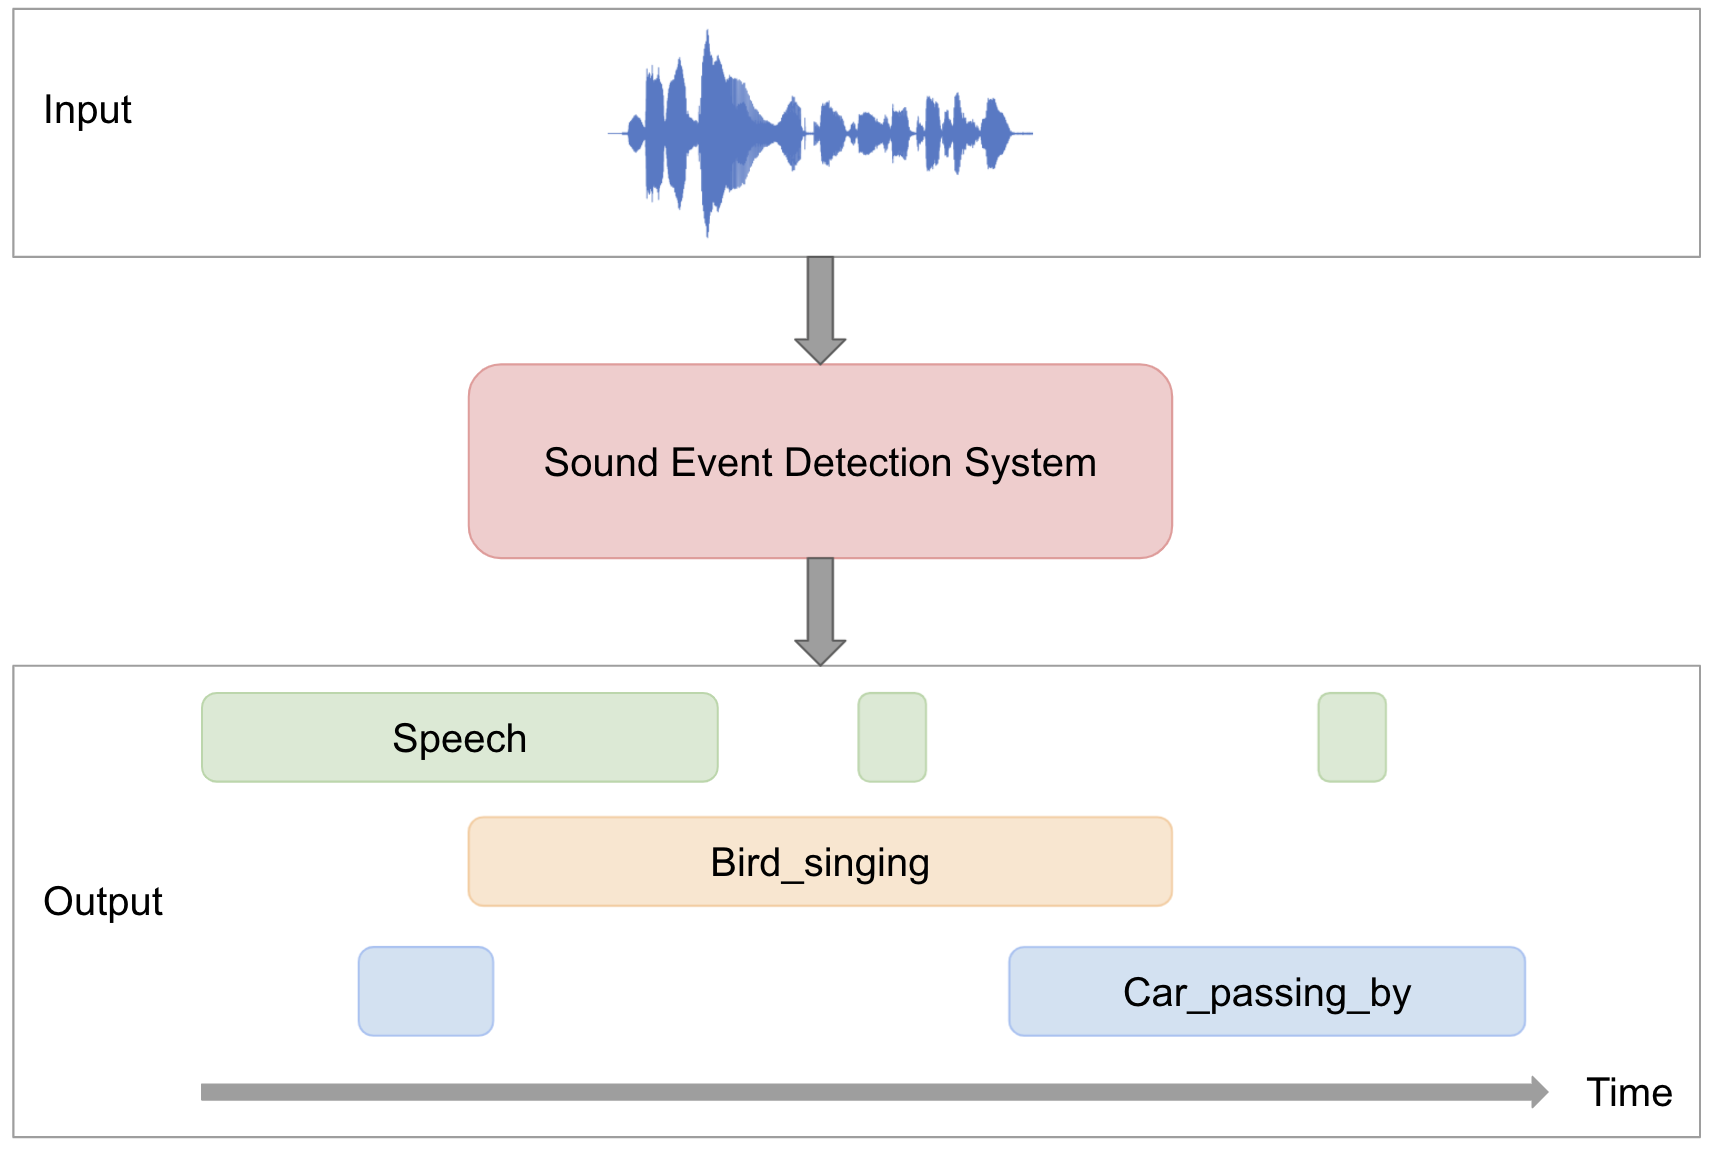
\includegraphics[width=\textwidth]{fig/sed-system.png}
    \caption{Overview of sound event detection system structure}
    \label{fig:sed-system}
\end{figure}

\begin{figure}[!htb]
    \centering
    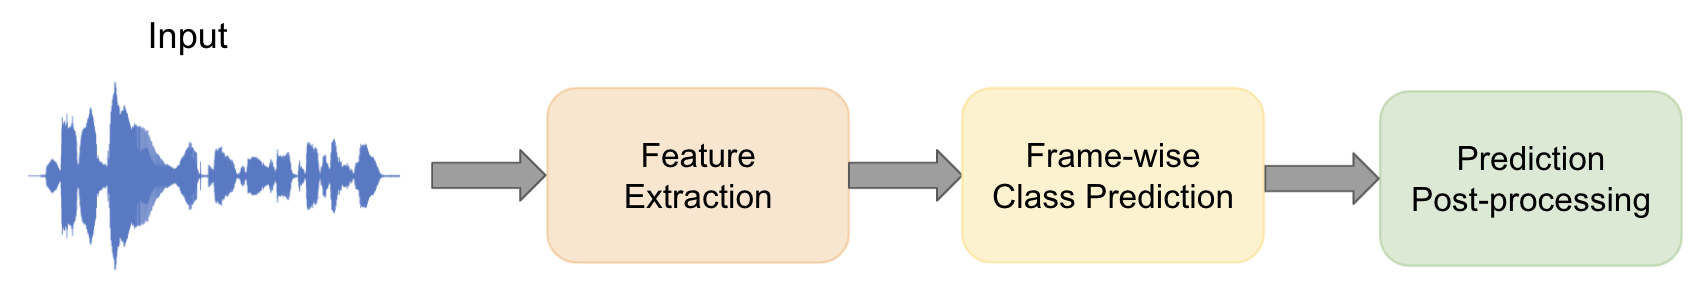
\includegraphics[width=\textwidth]{fig/sed-structure.png}
    \caption{Overview of sound event detection system}
    \label{fig:sed-structure}
\end{figure}

\section{SED Datasets}
This section introduces the common development datasets for SED tasks, as well as the novel dataset we curated for this project. Table \ref{tab:datasets} provides a summary of these datasets, most of which are from DCASE challenges. The audio clips in the DCASE datasets were recorded in real environments and released alongside the necessary meta information in WAV format.

\begin{table}[!htp]
\centering
\resizebox{\textwidth}{!}{\begin{tabular}{|c|c|c|c|c|c|c|c|}
\hline
\textbf{Dataset Name}                                                                                                                                       & \textbf{\begin{tabular}[c]{@{}c@{}}Year of \\ Release\end{tabular}}          & \textbf{\begin{tabular}[c]{@{}c@{}}Number \\ of Classes\end{tabular}} & \textbf{\begin{tabular}[c]{@{}c@{}}Total Audio\\ Duration\\ (Hours)\end{tabular}}     & \textbf{\begin{tabular}[c]{@{}c@{}}Segment\\ Length\\ (Seconds)\end{tabular}} & \textbf{\begin{tabular}[c]{@{}c@{}}Strongly\\ -labelled\end{tabular}}   & \textbf{\begin{tabular}[c]{@{}c@{}}Weakly\\ -labelled\end{tabular}}      & \textbf{Unlabelled}                                                    \\ \hline
\begin{tabular}[c]{@{}c@{}}DCASE 2020 Task 4\\ DCASE 2019 Task 4\\ DCASE 2018 Task 4\\ DCASE 2017 Task 4\\ DCASE 2016 Task 4\\ Project Dataset\end{tabular} & \begin{tabular}[c]{@{}c@{}}2020\\ 2019\\ 2018\\ 2017\\ 2016\\ -\end{tabular} & \begin{tabular}[c]{@{}c@{}}10\\ 10\\ 10\\ 17\\ 18\\ 25\end{tabular}   & \begin{tabular}[c]{@{}c@{}}51.59\\ 53.34\\ 45.22\\ 162.95\\ 1.88\\ 82.10\end{tabular} & \begin{tabular}[c]{@{}c@{}}10\\ 10\\ 10\\ 10\\ 10\\ 10\end{tabular}           & \begin{tabular}[c]{@{}c@{}}Yes\\ Yes\\ No\\ No\\ Yes\\ Yes\end{tabular} & \begin{tabular}[c]{@{}c@{}}Yes\\ Yes\\ Yes\\ Yes\\ No\\ Yes\end{tabular} & \begin{tabular}[c]{@{}c@{}}Yes\\ Yes\\ Yes\\ No\\ No\\ No\end{tabular} \\ \hline
\end{tabular}}
\caption{\label{tab:datasets}Sound event detection datasets}
\end{table}

 Most of these datasets, such as those from the DCASE 2017\cite{DCASE2017}, DCASE 2018 \cite{DCASE2018}, DCASE 2019 \cite{DCASE2019} and DCASE 2020 \cite{DCASE2019, Wisdom_InPrep2020} challenges, consist of a subset of the AudioSet dataset. AudioSet consists of 2,084,320 human-labelled 10-second audio clips extracted from YouTube videos and is made up of an ontology of 632 sound event classes  \cite{audioset}. There are two types of annotated data these datasets generally contain, namely strongly-labelled data and weakly-labelled data. The strongly-labelled data contains the specific onset and offset timestamps of when the sound events occur in a particular audio clip, while the weakly-labelled dataset only contains the tag information, which refers to the sound events that occur in a particular audio clip. Figure \ref{fig:weak-vs-strong} shows a comparison between strongly-labels and weakly-labels of an audio clip.\\

\begin{figure}[!htb]
    \centering
    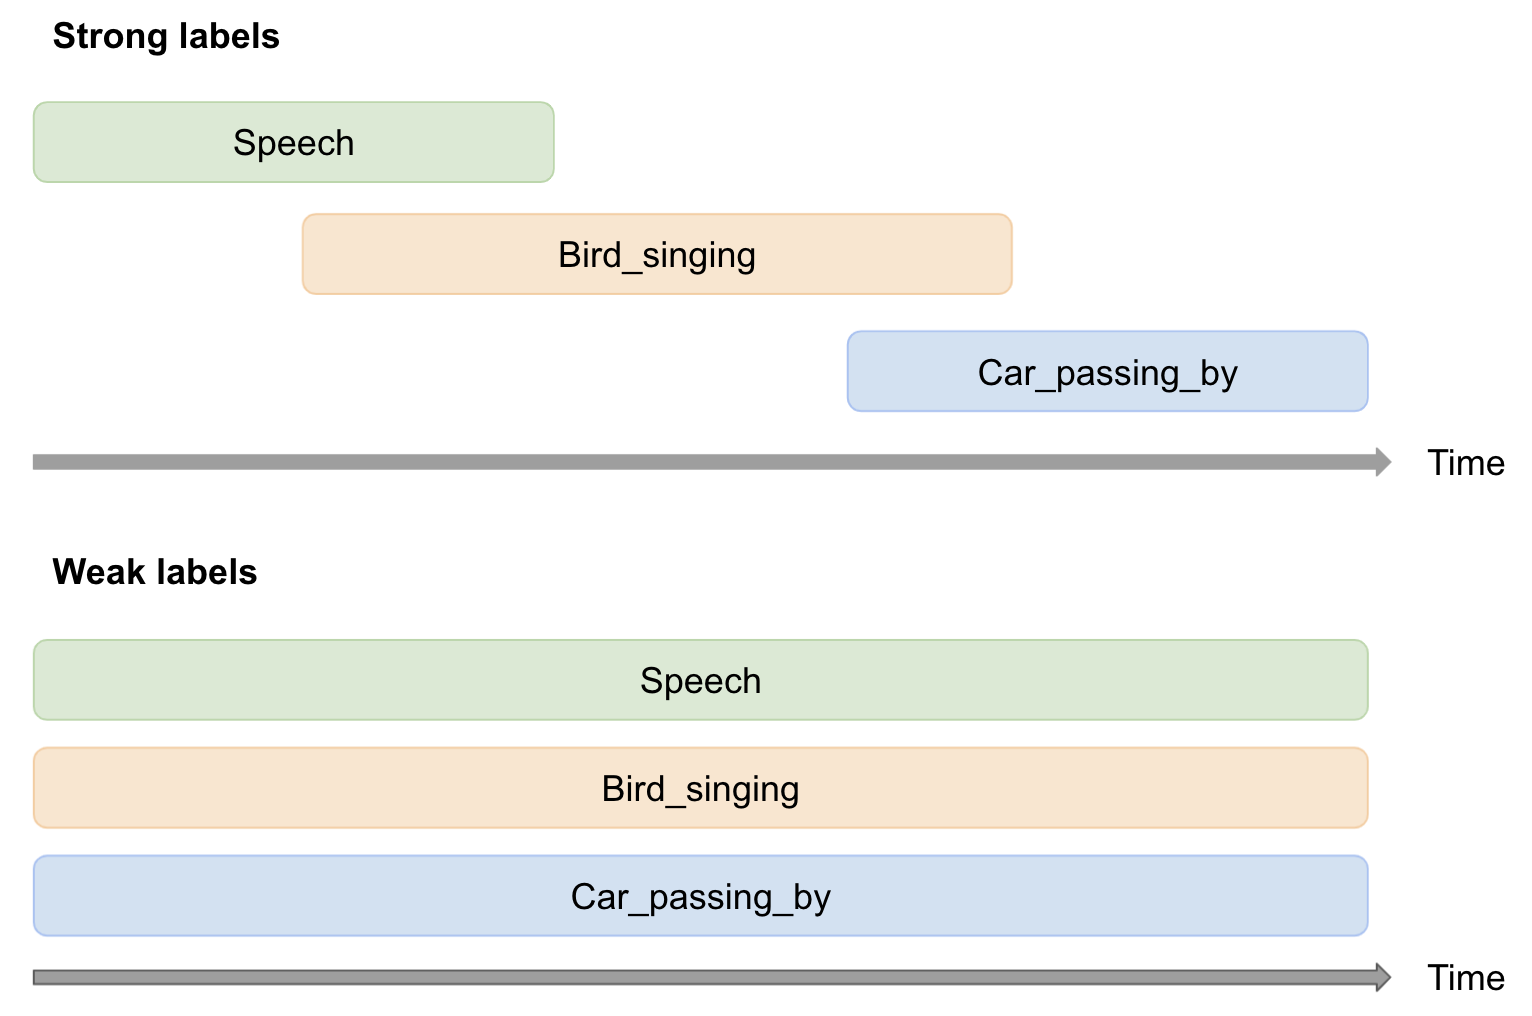
\includegraphics[width=\textwidth]{fig/weak-vs-strong.png}
    \caption{Comparison between strongly-labelled and weakly-labelled data}
    \label{fig:weak-vs-strong}
\end{figure}

% AudioSet is made up of an ontology of 632 audio event classes and a collection of 2,084,320 human-labelled 10-second sound clips extracted from YouTube videos \cite{audioset}. The ontology is a hierarchical graph of event categories which covers a wide range of human and animal sounds, musical instruments and genres, and everyday environmental sounds. The DCASE 2016 dataset \cite{DCASE2016} contains the highest number of sound event classes at 18, followed by DCASE 2017 \cite{DCASE2017} with 17 classes, then DCASE 2018 \cite{DCASE2018}, DCASE 2019 \cite{DCASE2019}  and DCASE 2020 \cite{DCASE2019, Wisdom_InPrep2020} with 10 classes. 
% The datasets also differ in terms of the types of data they contain. DCASE 2016 contains only strongly-labelled data while DCASE 2017 is only made up of weakly-labelled data. The remaining datasets contain a mix of data types. DCASE 2018 consists of unlabelled and weakly-labelled data while both DCASE 2019 and DCASE 2020 contain unlabelled, weakly-labelled and strongly-labelled data. 
% These DCASE challenges have provided a diverse set of sound event detection datasets and motivated many publications that have been evaluated with these datasets. 

In addition to these standard datasets provided by the DCASE challenges over the years, we have also curated our own dataset for this project in order to develop an SED system that is able to fulfil the requirements provided by our collaborating partner, DSO National Laboratories. The dataset is a subset of AudioSet \cite{audioset}, consisting of audio clips from 25 sound event classes related to human and emergency sounds, which is the highest number of sound event classes out of all the datasets discussed so far. The curation process and detailed information of this dataset will be discussed in Section 3.1. In this thesis, the SED system we developed is also evaluated with the DCASE 2017 dataset.

% The dataset is made up of a subset of the AudioSet dataset \cite{audioset}, focusing specifically on human sounds and emergency sounds, and incorporates the recently released strongly-labelled annotations for a subset of AudioSet \cite{hershey2021benefit}.

\section{Audio Features}
As the raw waveform data from audio clips cannot be understood by neural networks directly, feature extraction is needed to convert them into an understandable format. There are variety of audio feature types, most of which are spectrogram-based. However, no single feature type has yet proven complete superiority over the others for all SED tasks. A  spectrogram  is  a  visual  representation  of  the  spectrum  of  frequencies  of sound as they vary with time. These spectrogram representations have higher resolution and contain more information than general frame-based approaches \cite{spec-2019}, in terms of both temporal and frequency dimensions. This thesis focuses on the usage of log-mel and gammatone spectrogram representations. 

% These spectrograms are extracted from the audio clips and fed as input for training, instead of the raw audio clips themselves.

\subsection{Log-mel Spectrograms}
Log-mel spectrograms \cite{hershey2017cnn} are spectrogram representations that are derived from the classic spectrogram by applying a weighted average of the absolute values squared of the Short-Term Fourier Transform (STFT). They have been the most commonly used type of spectrogram representation in SED and Acoustic Scene Classification literature \cite{kong2020sound, Miyazaki2020CONFORMERBASEDSE, const_thres}, especially in conjunction with Convolutional Neural Networks (CNNs). It visualizes sounds on the Mel scale rather than the frequency domain, with log magnitude applied. The mel scale is a logarithmic transformation of a signal’s frequency. The basis of the idea of this transformation is that sounds of equal distance on the mel scale are perceived to be of equal distance to humans \cite{mel-scale}. This means that it is better able to mimic our own perception of sound. A mel spectrogram can be defined as:
\begin{equation}
MS_g(f)(b, v) = \sum_k|F(f \cdot T_bg)(k)|^2 \cdot \Lambda_v(k),
\end{equation}

where \(f\) represents the input signal, \(g\) is the window function for generating the spectrogram, and \(\Lambda_v\) is the mel-filters for \(v \in I = {1, . . . , K}\), where \(K\) is the chosen number of filters. The steps for computing log-mel spectrograms are as follows:
\begin{enumerate}
\item{Sample the input with Hann windows of \(x\) size, making hops of \(y\) size each time to sample the next window. The values of \(x\) and \(y\) are pre-defined.}
\item{Map each window from time domain to frequency domain by using the Fast Fourier Transform (FFT) algorithm.}
\item{Generate a mel scale by taking the entire frequency spectrum, and separating it into \(z\) bins evenly spaced frequencies. The mel scale values are calculated as follows:
\begin{equation}
    m = 2595 log_{10}(1 + \frac{f}{100})
\end{equation}}
\item{Generate the spectrograms by decomposing the magnitude of the signal into its components, corresponding to the frequencies in the Mel scale, for each window. }
\item{Apply the logarithmic conversion of the powers at each of the mel scale frequencies.}
\end{enumerate}

\subsection{Gammatone Spectrograms}
Gammatone spectrograms \cite{gammatone} are generated using gammatone filter-banks. Although they are not as commonly used as log-mel spectrograms, the gammatone filter have been designed to provide a closer approximation to the bandwidths of filters human auditory system \cite{slaney} and thus should provide an efficient representation. A Gammatone filter can be defined as:

\begin{equation}
g_{f_c}(t) = t^{N-1}exp(−2{\pi}tb(f_c)) cos(2πf_ct + {\phi})u(t),  
\end{equation}

where N represents the filter order, \(f_c\) is the filter center frequency in Hz, and \(\phi\) is the phase. \(u(t)\) is the unit step function which is \(u(t) = 1\) for \(t \geqslant 0\) and 0 otherwise. \(b(f_c)\) is the bandwidth of the filter. Empirical evidence has shown that \(N = 4\) provides a good match to the human auditory filter shape \cite{deliang}. The bandwidth of a gammatone filter used to model the human auditory system is generally chosen to be \(b(f_c) = 1.019 ERB(f_c) \approx 24.7(4.37f_c + 1)\). These filters are represented by an impulse response that is the product of a gamma distribution and sinusoidal tone. The impulse response of a 8 channel filter-bank is shown in Figure \ref{fig:impulse-frequency}(a) \cite{abdulla-gammatone}. The gammatone filter-bank is made up of a set of gammatone filters, which are channels with different centre frequencies. This is done to obtain a representation similar to a FFT-based spectrogram. An example of the frequency response of a 8 channel filter-bank is shown in Figure \ref{fig:impulse-frequency}(b) \cite{abdulla-gammatone}.\\

\begin{figure}[!htp]
    \centering
    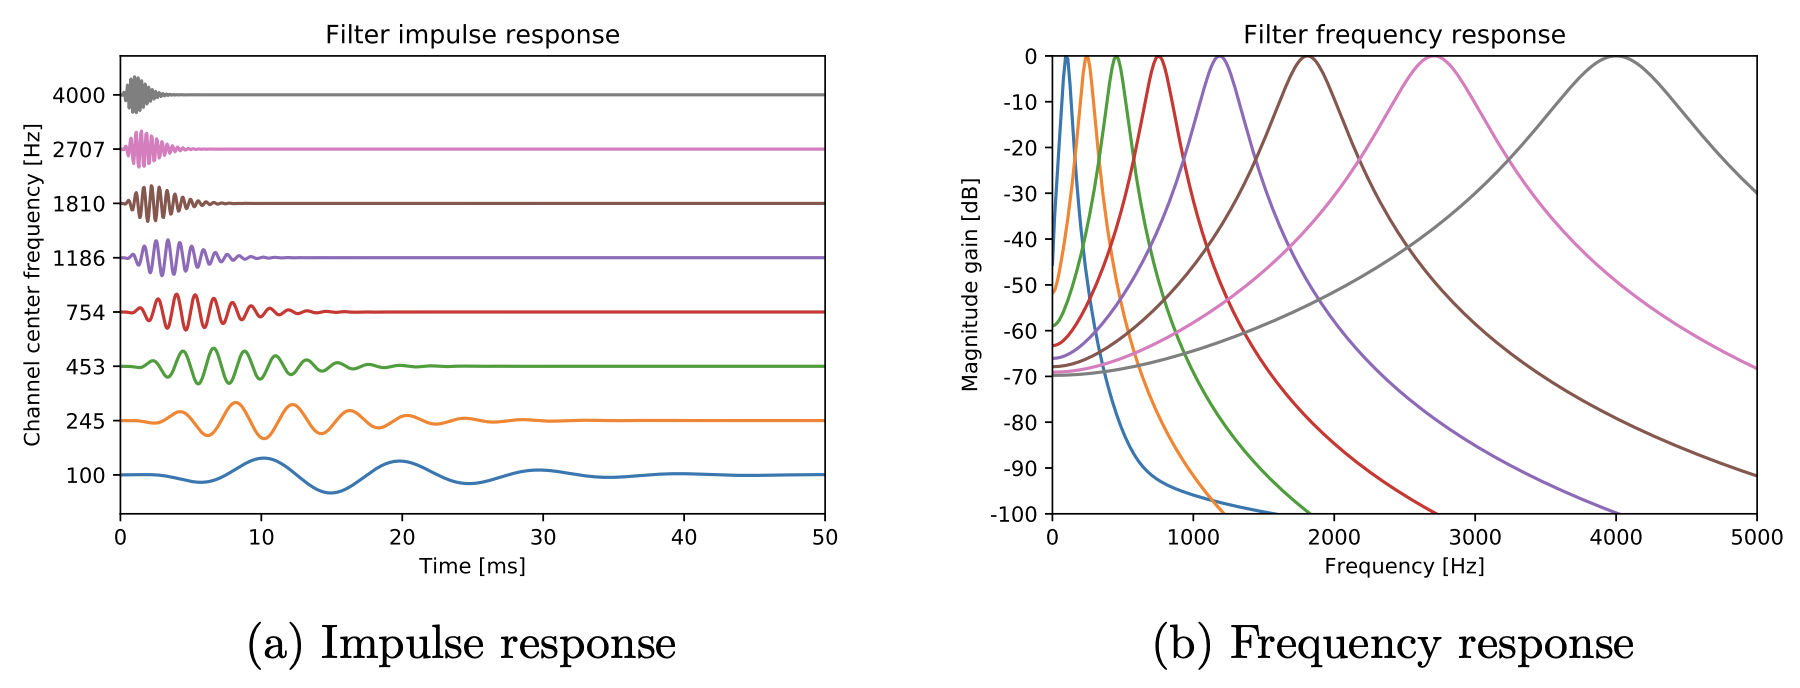
\includegraphics[width=\textwidth]{fig/impulse_frequency.png}
    \caption{Impulse (a) and frequency (b) response of a 8-channel filterbank, centered at equally spaced points between 100 Hz and 4 kHz
on the ERB scale}
    \label{fig:impulse-frequency}
\end{figure}

% \begin{figure}[!htb]
%     \centering
%     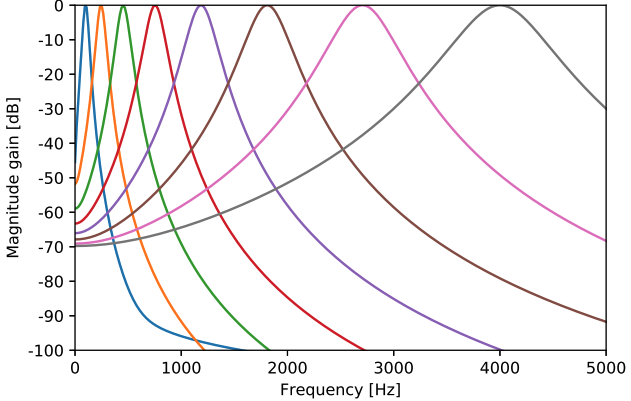
\includegraphics[width=0.7\textwidth]{fig/frequency-response.png}
%     \caption{Frequency response of a 8-channel filterbank, centered at equally spaced points between 100 Hz and 4 kHz
% on the ERB scale}
%     \label{fig:frequency-response}
% \end{figure}

% A set of gammatone filters, which are channels with different centre frequencies, is used to create the gammatone filter-bank. This is done to obtain a representation similar to a FFT-based spectrogram. An example of the frequency response of a 8 channel filter-bank is shown in Figure \ref{fig:frequency-response} \cite{abdulla-gammatone}.\\

The steps for computing gammatone spectrograms are as follows:

\begin{enumerate}
\item{Sample the input with Hann windows of \(x\) size, making hops of size \(y\) each time to sample the next window. The values of \(x\) and \(y\) are pre-defined.}
\item{Compute the Discrete Fourier Transform (DFT) for each window \(a^t\):
\begin{equation}
A^t_k = \sum^{n−1}_{m=0}a^t_m exp(−2{\pi}i\frac{mk}{n}), \quad k = 0, . . . , n - 1.
\end{equation}

The output of the DFT is Hermetian symmetric since the input windows are real-valued. Thus, the negative-frequency terms are redundant and can be removed. Since the first bin \(A^t_0\) contains the zero-frequency term of the signal, it is also removed. As a result, \(\frac{n}{2}\) points \(A^t = [A^t_1, A^t_2, ..., A^t_\frac{n}{2}]^T\) are left for each window.
\item{Compute the square of the absolute value of each window component. Stack the resulting vectors to obtain the power spectrogram A:
\begin{equation}
A = [|A^1|^2, |A^2|^2,  ..., |A^t|^2]
\end{equation}}
\item{Weight each bin \(|A^i|^2\) of the power spectrogram according to the expected magnitude gain of a gammatone filter of the same centre frequency corresponding to the DFT bin. This can be expressed by the matrix multiplication \(G = W A\). W is computed by transforming the impulse response of m gammatone filters evenly spaced on the ERB scale using an n-point DFT.
\begin{equation} W = 
\begin{bmatrix}
|DFT{g_{f1}(t)|^2\\
|DFT{g_{f2}(t)|^2\\
\vdots\\
|DFT{g_{fm}(t)|^2
\end{bmatrix}
\end{equation}}
\item{Apply the logarithmic conversion of the powers at each of the frequencies.}
\end{enumerate}

\section{Data Augmentation Techniques}
In the audio domain, data augmentation is used to artificially generate new data through data manipulation in order to improve generalisation and performance \cite{Wei_2020}. Although there are a variety of data augmentation techniques available, the authors Kong et al. \cite{kong2020sound} and Miyazaki et al. \cite{Miyazaki2020CONFORMERBASEDSE}, mainly focused on SpecAugment \cite{specaugment}, mixup \cite{mixup} and time-shift \cite{timeshift}, and managed to successfully produce the best-performing models for the DCASE 2017 and DCASE 2020 SED tasks respectively. As such, we will only focus on the aforementioned techniques in this thesis.

\subsection{SpecAugment}
Park et al. \cite{specaugment} developed SpecAugment to be used as a simple data augmentation technique for speech recognition tasks. The augmentation policy includes frequency-masking and time-masking. Figure \ref{fig:specaugment} shows a comparison between the original, frequency-masked, and time-masked audio.\\

\begin{figure}[!htb]
    \centering
    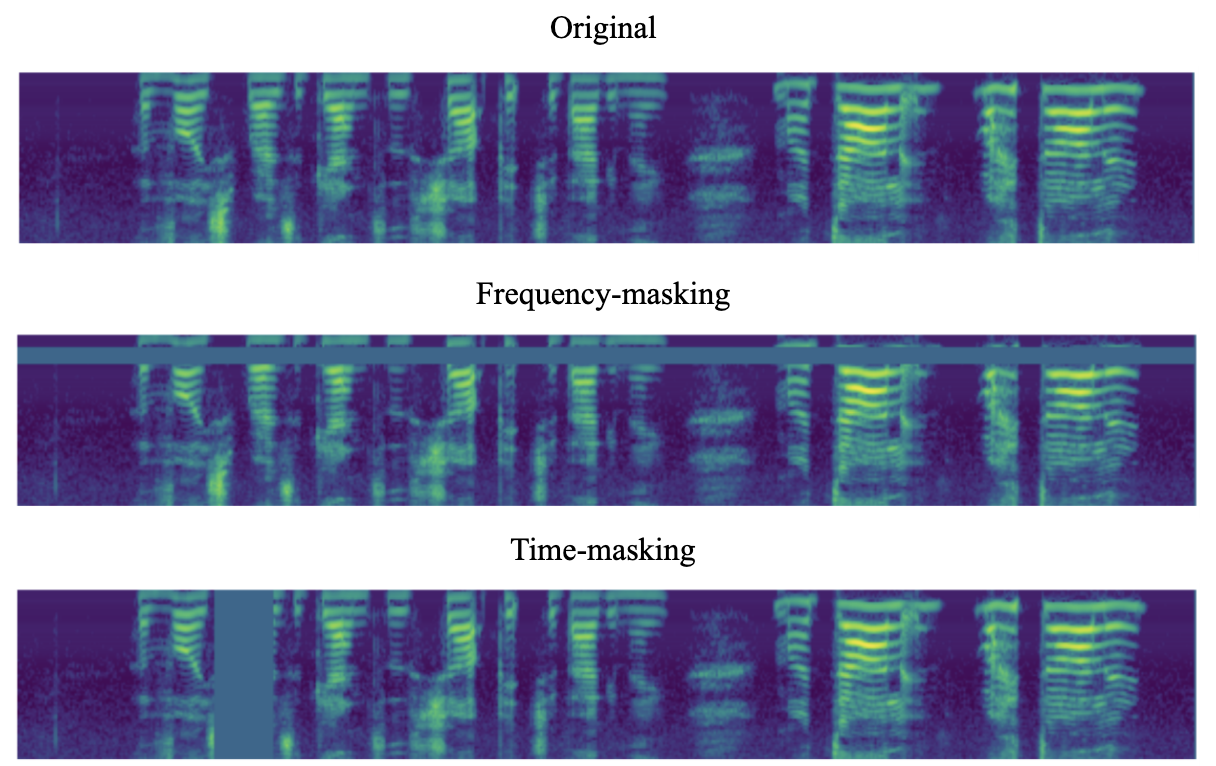
\includegraphics[width=\textwidth]{fig/specaugment.png}
    \caption{Comparison between original, frequency-masked and time-masked audio}
    \label{fig:specaugment}
\end{figure}

 In frequency masking, the frequency channels \([f_0, f_0 + f)\) are masked, which is done by replacing the corresponding values with zeroes. \(f\) is chosen from a uniform distribution between 0 and the frequency mask parameter \(F\), and \(f_0\) is chosen from \((0, v - f)\) where ν is the number of frequency channels. \\

Time masking replaces values in the time domain with zeroes, such that \(t\) consecutive time steps \([t_0, t_0 + t)\) are masked, where \(t\) is first chosen from a uniform distribution from 0 to the time mask parameter \(T\), and \(t_0\) is chosen from \([0, \tau - t)\), where \(\tau\) is the number of time steps.

\subsection{Mixup}
Zhang et al. \cite{mixup} originally developed mixup for computer vision tasks but its use has since been extended to the audio domain. Mixup smooths out the decision boundary by adding pseudo data generated by mixing different data points and the corresponding labels. By doing so, mixup regularizes the neural network to favour simple linear behavior in between training examples. Additionally, mixup has been found to decrease the memorization of corrupt labels, raise the robustness against adversarial examples, and stabilize the training of generative adversarial networks \cite{thulasidasan2020mixup}. Mixup can be represented in the following equation \ref{eqn:mixup-1} and \ref{eqn:mixup-2}:

\begin{align}
\label{eqn:mixup-1}
x¯ = \lambda{x_1} + (1 - \lambda)x_2,\\
\label{eqn:mixup-2}
y¯ = \lambda{y_1}+ (1 - \lambda)y_2,
\end{align}

where \((x_1, x_2)\) and \((y_1, y_2)\) represent different data points and their corresponding labels, respectively, and \(\lambda\) is the mixing \(\in\) [0,1]. In mixup, the \(\lambda\) value denotes the degree of mixing between the spectrograms. For instance, when mixup is applied on two spectrograms tagged with different sound events, the output spectrogram is a blend of the original two \cite{mixup_ex}. An example of mixup is shown in Figure \ref{fig:mixup}.

\begin{figure}[!htb]
    \centering
    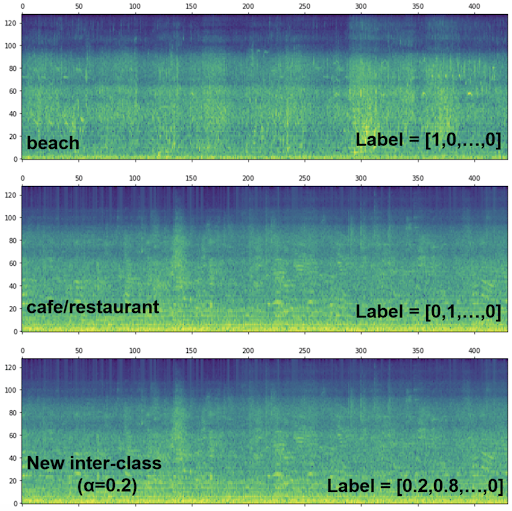
\includegraphics[width=0.8\textwidth]{fig/mixup.png}
    \caption{Example of mixup audio product}
    \label{fig:mixup}
\end{figure}

\subsection{Time-shift}
In time-shifting \cite{timeshift}, a feature sequence is shifted along the time axis, with the overrun frames being concatenated with the opposite end of the sequence. As reported in \cite{Miyazaki2020CONFORMERBASEDSE}, time-shifting has shown to help prevent the model from learning bias in time event localization. Figure \ref{fig:timeshift} shows a comparison between the original and time-shifted audio.

\begin{figure}[!htb]
    \centering
    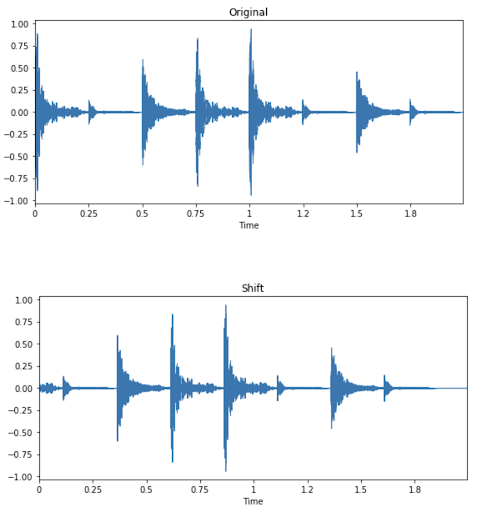
\includegraphics[width=0.8\textwidth]{fig/time-shift.png}
    \caption{Comparison between original and time-shifted audio}
    \label{fig:timeshift}
\end{figure}

\section{Deep Learning Approach}
The general approach to tackle the SED task is based on supervised learning, where a training set of audio recordings and their reference annotations of class events are used to learn an acoustic model. Early approaches for SED employed techniques from speech recognition and music information retrieval. These approaches were based on traditional pattern classification techniques such as Gaussian mixture models (GMMs) and hidden Markov models (HMMs). Notably, in 2007, Chien et al. \cite{Chien_2007} utilised GMMs for wheeze detection, and Schmidt et al. \cite{Schmidt_2010} employed HMMs to segment heart sound recordings in 2010. However, due to specific methods that allow the modelling of elementary units in speech or music, such as state-tying of phonemes or left-to-right topologies for modeling temporal evolution of phonemes and musical notes, GMMs and HMMs models are much more useful in speech and music modeling. Furthermore, sound events generally do not consist of similar elementary units as speech. This makes GMMs and HMMs less relevant for SED tasks. In addition, these models are not designed to detect multiple classes at the same time, making them unsuitable for polyphonic SED tasks. In order to solve the multi-label classification problem, they utilised extensions or setups, such as binary classification for each sound event class \cite{Mesaros2016TUTDF}, or multiple passes of Viterbi decoding \cite{heittola-2013} or pre-processing involving sound source separation \cite{heittola-2011}.\\ 

In contrast, modern pattern classification tools, especially deep neural networks (DNNs), can perform multi-label classification much more easily, as demonstrated by Cakir et al. \cite{Cakir_2015} in 2015. This is because multiple output neurons being active at the same time indicate the activity of multiple sound classes at the same time. This gives DNNs a great edge in solving the multi-label classification problem, and has made them predominant in the field. The utilisation of DNNs in SED tasks has allowed for major advancements in the field, with systems achieving state-of-the art performance and gaining the ability to tackle more complex problems.

\subsection{Convolutional Neural Network (CNN)}
CNNs were originally developed for image classification \cite{NIPS2012_cnn} but its usage has since been extended to audio related tasks such as sound event detection \cite{kong2020sound}, speech recognition \cite{cnn-asr} and audio tagging \cite{cnn-at}. Although we can construct an SED system purely from a CNN, its limited receptive field size means that it is unable to capture long time dependency in an audio clip. This is detrimental when analysing sound events that have long time dependencies. For example, a siren from an emergency vehicle may last for many seconds or even minutes. To allow the model to better capture the temporal dependency, Xu et al. \cite{xu2017convolutional} and Miyazaki et al. \cite{Miyazaki2020CONFORMERBASEDSE} have found that combining CNNs with other model types, such as RNNs, transformers and conformers allows the network to better extract the global and local context information from a feature sequence. This in turn makes for a better performing SED system.\\

A standard CNN comprises of convolution layers, pooling layers and fully connected layers. Each convolutional layer contains a set of learnable kernels, and its output is a tensor known as a feature map. These kernels are able to learn the local time-frequency patterns in the spectrogram extracted from an audio clip. In audio processing, the low level features \cite{thickstun2017learning} can be the raw wave-forms or spectrograms. The high level features are then extracted by the convolutional layers from these low level features. Following recent CNN architecures, batch normalization \cite{ioffe2015batch} is then applied after the convolutional layers to stabilise and increase the speed of training. After each batch normalization, non-linear activation functions, such as ReLU \cite{relu}, are then applied. For SED tasks, pooling layers are also applied along both time and frequency axes. Finally, the output of the last convolutional layer is fed as input to a time-distributed fully connected layer in order to predict the presence probability of sound events along the time axis. 

\subsection{Recurrent Neural Network (RNN) Based Models}
% As the receptive field of CNNs have limited sizes, this means that CNNs are unable to capture long time dependency in an audio clip. However, some sound events may have long time dependencies. For example, a siren from an emergency vehicle may last for many seconds or even minutes. In cases like these, temporal information would be especially useful for SED. Therefore, developing a system that is able to capture the temporal dependency, such as a CRNN \cite{xu2017convolutional}, is beneficial for SED tasks. 

Recurrent neural networks (RNNs) \cite{Mikolov:2010wx} are a type of neural network that can capture the long-term dependency of sequential data by storing history information in their hidden states. In fact, RNNs are frequently utilised in natural language processing tasks and have been shown to perform well in them \cite{devlin2019bert}. However, a possible problem with standard RNNs is that the gradient of the weights may vanish or explode during training. To prevent the gradient from exploding and vanishing, Long short term memory (LSTM) \cite{hochreiter1997long} systems have been developed. LSTMs are a variation of RNN and they comprise of constant error carousel units, input gate, output gate and forget gate. Notably, LSTMs have shown great promise in SED task, with Wang et.al \cite{Wang_2016} achieving better frame-wise performance through the use of it. LSTMs have also been further improved in the form of Gated Recurrent Units (GRUs) \cite{cho2014learning}. GRUs reduce the parameters of LSTMs and simplify the gates to a reset gate and a forget gate. Additionally, GRUs can be in both directions, which is known as a bidirectional GRU. In fact, Kong et al. \cite{kong2020sound} was able to achieve state-of-the-art performance for the DCASE 2017 SED challenge with the use of a bi-directional GRU, combined with a CNN, in his system. 
% Of the different variations of RNNs, we mainly experimented with the bi-directional GRUs in our thesis.

\subsection{Transformer-Based Models}
The transformer was originally proposed by Vaswani et al. \cite{vaswani2017attention} in 2017, and its design was motivated by the goal of allowing dependencies to be modelled without the consideration of their distance in the input sequence. In comparison to RNNs, the absence of recurrent connections in transformers allows for more parallel computing, which gives it slight advantage in terms of training speed. Transformers have mainly been applied in natural language processing tasks, but its use has since been extended to SED tasks, with good performance reported in \cite{kong2020sound}. However, Miyazaki et al. \cite{Miyazaki2020CONFORMERBASEDSE} has found that transformers are less effective in capturing local context information, which is essential for SED, in comparison to the more recently proposed Conformer model \cite{gulati2020conformer}.\\ 
 
A typical transformer may comprise of several encoder and decoder layers. When an input is fed into a transformer, it is transformed into a high level embedding by the encode, which can then be transformed to an output by the decoder. In SED tasks, only the encoder is required, and each encoder is made up several encoder layers. The encoder layer contains a query transform matrix \(W^Q\), a key transform matrix \(W^K\) and a value transform matrix \(W^V\). The matrices \(W^Q\) and \(W^K\) have a shape of \(C × d_k\), and \(W^V\) has a shape of \(C \times d_v\), where \(C\) represents the number of channels, and \(d_k\) and \(d_v\) are integers. Then the query \(Q\),  key \(K\) and value \(V\) can be obtained by:

\begin{align}
Q = xW^Q\\
K = xW^K\\
V = xW^V 
\end{align}

The query Q and key K have a shape of \(T \times d_k\), and the value \(V\) has a shape of \(T \times d_v\), where \(T\) refers to the number of time steps. The output of an encoder layer can be written as: 

\begin{equation}
\label{eqn:trans-4}
h = softmax(\frac{QK^T}{\sqrt{d_k}})V ,
\end{equation}

where the output \(h\) has a shape of \(T \times H\). In equation \ref{eqn:trans-4}, the division of the square root of \(d_k\) is a normalization term \cite{vaswani2017attention}, and the inner product of \(Q\) and \(K^T\) has a shape of \(T \times T\), which represents the feature correlation of different time steps. The softmax function transforms the correlation value to probabilities along the time steps, which indicate how much the value \(V\) in a time step should be attended to.

\subsection{Conformer-Based Models}
The conformer was originally proposed by Gulati et al. \cite{gulati2020conformer} in 2020. It is essentially a convolution-augmented Transformer. By combining self-attention with a CNN, it is able to achieve high performance and efficient parameter reduction. This is possible because it is able exploit the strengths of each component, that is, self-attention is better at modeling long-range, global context information, while CNNs are better at extracting local features. The conformer has been reported to achieve state-of-the-art performance in automatic speech recognition (ASR) and SED. Specifically, Miyazaki et al. \cite{Miyazaki2020CONFORMERBASEDSE} was able achieve the best-performing model for the DCASE 2020 Task 4 with the use of conformers in his system, with it slightly outperforming the transformer system he tested in his study as well.\\

The conformer block is made up of three modules, namely a feed-forward module, a multi-head self-attention module, and a convolution module. The feed-forward module comprises of a layer-normalization layer, a linear layer with a Swish activation function \cite{ramachandran2017searching}, which expands the dimensions of the input by four times, and finally another linear layer, which projects the dimensions back to those of the original input. The multi-head self-attention module contains a layer-normalization and multi-head self-attention with relative positional embedding, as used in Transformer-XL \cite{dai-etal-2019-transformer}. The convolution module is made up of a layer normalization layer, a point-wise convolution layer with a gated linear unit (GLU) activation function \cite{dauphin2017language}, and a 1-D depth-wise convolution layer, which is then followed by a batch normalization layer, Swish activation, and finally a point-wise convolution layer. The relation between the input \(X\) and output \(Y\) of the conformer block can thus be modelled as follows:

\begin{align}
X˜ = X + \frac{1}{2}FFN(X),\\
X` = X˜ + MHSA(X˜),\\
X`` = X` + Conv(X),\\
Y = LayerNorm(X`` + \frac{1}{2}FFN(X``)),  
\end{align}

where \(FFN(\cdot)\), \(MHSA(\cdot)\), \(Conv(\cdot)\), and \(LayerNorm(\cdot)\) refer to the feed-forward module, multi-head self-attention module, convolution module, and layer-normalization layer, respectively.

\subsection{Transfer Learning}
% % Transfer learning is a machine learning method where a model developed for a particular task is reused as the starting point for a model on a second task \cite{trans-learn}. With transfer learning, we can train a deep neural network with comparatively little data. 

In transfer learning, the knowledge of a pre-trained model is applied to a different but related problem \cite{trans-learn}. This is done to exploit what has been learned in one task to improve the generalisation of another. As such, transfer learning has the potential to speed up training and improve the performance of a neural network model. In fact, Jung et al. \cite{Jung_2019} reported a significant improvement in the performance of his SED system through the integration of transfer learning with his model.\\ 
% % In deep learning we transfer weights that a network has learned in one task to another. If the source and target data are similar, then the knowledge can be transferred from a high number of source layers. We will be exploring the use of transfer learning methods for CNN as it has proven to be useful \cite{trans-learn-2019}.\\ 

There are two main transfer learning strategies that can be applied, which are summaried in Figure \ref{fig:transfer-learning}. The first strategy is to use the pre-trained model as a feature extractor, with no further training done. In the context of the SED task, this means that the embedding features of audio clips are first calculated with the pre-trained model. These embedding features are later used as input to a classifier. When training on the new dataset, the parameters of the pre-trained model are frozen and not trained, and only the parameters of classifier built on embedding features are trained. This strategy is typically only used when the new dataset and the dataset the model was pre-trained on are similar. In contrast, the second strategy is to fine-tune the pre-trained model with the data from the new task. This involves initialising all the parameters from the pre-trained model, except final fully-connected layer. These parameters are then further trained on the dataset of the new task.

\begin{figure}[!htp]
    \centering
    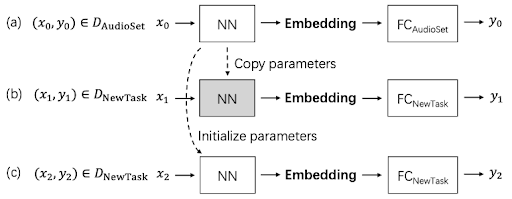
\includegraphics[width=\textwidth]{fig/transfer-learning.png}
    \caption{Transfer learning strategies. (a) represents the pre-trained model. (b) is the pre-trained model being using as a feature extractor. (c) is where the pre-trained model is fine-tuned on the new dataset.}
    \label{fig:transfer-learning}
\end{figure}

\section{Automatic Threshold Optimisation}
The threshold values play an important role in prediction post-processing in SED tasks. That is, if the predicted probability that a certain sound event is present in a frame exceeds the threshold value, then the frame is regarded to contain this sound event. The selection of the threshold values for post-processing is a challenging problem. They are typically manually selected, and are commonly set to 0.5 for most SED systems \cite{const_thres}. However, these threshold values are usually not optimal for all the sound event classes. As such, the selection of threshold values is an important part of SED tasks as incorrect selection may have detrimental effects on the performance of a SED system. In order to solve this problem, Kong et al. \cite{kong2020sound} has proposed an automatic threshold optimisation method to determine the optimal threshold values for different sound event classes. The automatic threshold optimisation method optimises thresholds based on a metric such as F1-score, and  has been found to improve the performance of SED systems. Hence, we will be experimenting with the use of automatic threshold optimisation in this thesis since it has been proven to be useful in similar tasks.

\section{Open Issues}
Existing literature on SED, specifically for the recent DCASE SED challenges, have mainly developed systems to analyse audio clips as a whole and have yet to explore the impacts of applying rolling segmentation windows on the audio clips prior to analysis. This is in spite of the fact that doing so may yield potential benefits, especially in real-life applications. In real-life applications, the audio clips we would usually like to analyse could be hours long. Therefore, processing these long audio clips as a whole is not feasible as it is online and on the fly. As such, they are usually divided into segments of \(x\) seconds and fed into the system for analysis. However, just purely dividing the audio clips into non-overlapping segments and sending them for analysis may not yield the best outcome. This is because depending on the segment length or the temporal position where the audio clip is partitioned and sent to the system for analysis, the SED system may output slightly different results. For edge cases, such as sound events occurring right at the end of one segment and continuing over to the succeeding segment, the SED system may not even be able to detect them as the sound event is broken apart and not analysed as a whole. In this thesis, we will explore this issue and propose some methods, such as averaging frame-wise predictions, to remedy it.

% Existing literature on SED have only focused on developing systems to have optimised performance on the common SED datasets mentioned in Section 2.2, whose evaluation sets only consist of 10 second long audio clips, and have overlooked optimising their performance on clips with long audio duration. However, in real-life applications, the audio clips we would usually like to evaluate on could be hours long. Processing these long audio clips as a whole is not feasible as it is online and on the fly. Therefore, they are usually divided into segments of \(x\) seconds and fed into the system for analysis. Depending on the segment length or the temporal position where the audio clip is portioned and sent to the system for analysis, the SED system may output slightly different results. For edge cases, such as sound events occurring right at the end of one segment and continuing over to the succeeding segment, the SED system may not even be able to detect them as the sound event is broken apart and not analysed as a whole. In this thesis, we will explore this issue and propose some methods, such as averaging frame-wise predictions, to remedy it.

% The issues of how an audio clip recording should be segmented before being sent to the SED system to be analysed, and how it should be processed after, is often overlooked in scientific publications. This is especially important when analysing clips with long audio durations.  


%=== END OF LITERATURE REVIEW ===
\newpage
\lhead{Proposed Approach and System Specifications}
\linespread{1.3}
\chapter{Dataset Curation, Proposed Approach and Specifications}

\section{Dataset Curation}
The development dataset is a novel dataset we curated using a subset of AudioSet. The development set contains both weakly-labelled and strongly-labelled data, as it incorporates the recently released strongly-labelled annotations for a subset of AudioSet \cite{hershey2021benefit}. This dataset is made up of 29,556 audio files in total, with 25,834 audio clips in the weakly-labelled train set, 2,380 clips in the strongly-labelled train set, 595 clips in the strongly-labelled validation set, and 747 clips in the strongly-labelled test set. There are a total of 25 sound event classes which are divided into two main categories: human and emergency. Most of the audio clips are 10 seconds long. The audio clips which are shorter than 10 seconds are padded with silence to 10 seconds. Table \ref{tab:main-dataset} lists the sound events and their statistics. The development set includes audio clips from the training set and validation set.\\

\begin{table}[!htp]
\centering
\begin{tabular}{|c|c|c|c|}
\hline
\multirow{2}{*}{\textbf{Sound Type}} & \multirow{2}{*}{\textbf{Sound Event}}                                                                                                                                                                                                                                                                               & \multicolumn{2}{c|}{\textbf{\begin{tabular}[c]{@{}c@{}}Number of \\ Event Instances\end{tabular}}}                                                                                                                                                                                                           \\ \cline{3-4} 
                                     &                                                                                                                                                                                                                                                                                                                     & \textbf{Development}                                                                                                                                                  & \textbf{Test}                                                                                                                        \\ \hline
Human                                & \begin{tabular}[c]{@{}c@{}}Applause\\ Breathing\\ Chatter\\ Cheering\\ Child speech, kid speaking\\ Clapping\\ Conversation\\ Cough\\ Crowd\\ Crying, sobbing\\ Female speech, woman speaking\\ Laughter\\ Male speech, man speaking\\ Run\\ Screaming\\ Shout\\ Sneeze\\ Walk, footsteps\\ Whispering\end{tabular} & \begin{tabular}[c]{@{}c@{}}552\\ 161\\ 259\\ 1,138\\ 2,119\\ 155\\ 1,004\\ 182\\ 2,220\\ 339\\ 4,263\\ 1,381\\ 10,739\\ 522\\ 243\\ 44\\ 279\\ 645\\ 460\end{tabular} & \begin{tabular}[c]{@{}c@{}}25\\ 31\\ 21\\ 35\\ 48\\ 25\\ 37\\ 26\\ 94\\ 21\\ 20\\ 59\\ 20\\ 20\\ 15\\ 11\\ 21\\ 30\\ 30\end{tabular} \\ \hline
Emergency                            & \begin{tabular}[c]{@{}c@{}}Air horn, truck horn\\ Car alarm\\ Emergency vehicle\\ Explosion\\ Gunshot, gunfire\\ Siren\end{tabular}                                                                                                                                                                                 & \begin{tabular}[c]{@{}c@{}}94\\ 140\\ 1,630\\ 466\\ 917\\ 2,889\end{tabular}                                                                                          & \begin{tabular}[c]{@{}c@{}}19\\ 37\\ 106\\ 16\\ 33\\ 160\end{tabular}                                                                \\ \hline
\end{tabular}
\caption{\label{tab:main-dataset}Summary of sound events in project dataset}
\end{table}

% This dataset was curated with the aid of the YouTube-DL and FFmpeg \cite{tomar2006converting} packages. YouTube-DL enables the audio clips to be downloaded from YouTube efficiently, while FFmpeg extracts a portion of the downloaded audio clips and resamples them to the predefined sample rate. 
The curation of the dataset was done in three main stages. In the first stage, we made a list of labels of the 25 sound event classes we wanted the audio clips extracted from AudioSet to be tagged as. Since the AudioSet sound event labels is a collection of sound events organised in a hierarchy, an audio clip tagged with a ‘child’ label would also be tagged with the ‘parent’ label. For instance, an audio clip tagged with the ‘Applause’ or ‘Cheering’ label is also tagged with the ‘Human group actions’ label. As such, we included the corresponding ‘parent’ labels to each of the 25 classes in the aforementioned list of labels. In the second stage, we filtered the publicly available metadata of the AudioSet dataset to extract the names of the audio clips that were only tagged with labels present in the list of labels produced in stage 1. In the final stage, we used YouTube-DL to download the audio clips whose names are present in the filtered metadata, and then used FFmpeg \cite{tomar2006converting} to trim the downloaded audio clips in accordance with the start and end time stated in the metadata, and resample them to 16k Hz.

\subsection{Dataset with Lower Audio Quality}
In real-life scenarios, the audio quality of a recording that a user typically inputs into the SED system would be quite poor. It would be unwise to assume that their input audio clips would always be of similar quality to the clips in the development dataset. Therefore, we created a development dataset with lower audio quality in order to develop a SED system that performs well with inputs of lower audio quality. This is done by using pipe and FFmpeg to generate different types of codec effects on the higher quality audio clips and resample them to 8k Hz. 

\section{Proposed Methodology}
In this thesis, we experimented with different system structures which incorporate the different approaches discussed in Chapter 2. The main development dataset used in this project is novel and the data type combination it consists of is slightly different from that of the standard SED datasets mentioned in Section 2.2. The project dataset consists of both weakly-labelled and strongly-labelled data, with the weakly-labelled training set being around 11 times larger than the strongly-labelled training set. This is in contrast to the standard datasets, which can be fully strongly-labelled (DCASE 2016) or weakly-labelled (DCASE 2017), weakly-labelled and unlabelled (DCASE 2018), or strongly-labelled, weakly-labelled and unlabelled (DCASE 2019 and DCASE 2020). As such, previous works based on these standard datasets were not entirely applicable to our task at hand. Therefore, we took ideas from each of these approaches, as well as proposed a frame-wise prediction pre-processing and post-processing method, in order to develop a system that was appropriate for the dataset we had to work with and the intended purpose of our SED system, which is to analyse clips with long audio duration.\\ 

With regards to the audio features, related works mentioned in Section 2.3 have shown that both log-mel and gammatone spectrograms are viable options to be used as input for training the SED systems. Both spectrograms were designed to better mimic the human auditory system. Thus, we experimented with both types of spectrogram representations in our SED system.\\

For data augmentation techniques, previous works mentioned in Section 2.4 focused on SpecAugment, time-shifting and mixup. Although there are other data augmentation techniques that may be useful for processing the spectrogram representations before passing them as input for training, previous works in \cite{kong2020sound, Miyazaki2020CONFORMERBASEDSE} have made use of the aforementioned techniques specifically for SED tasks, even producing the best-performing models for the DCASE 2017 and DCASE 2020 Task 4 challenges. Hence, we focused our experiments on these three data augmentation techniques for our SED system.\\ 

For model architectures, related works shown in Section 2.5 focused on GRU-based, transformer-based and conformer-based neural networks. As these networks have shown to produce comparative results in \cite{kong2020sound} and \cite{Miyazaki2020CONFORMERBASEDSE}, we experimented with the aforementioned network architectures for our SED system in order to determine the best one for our project development dataset.\\

According to \cite{kong2020sound}, rather than using manually-selected thresholds values, employing optimised threshold values determined from automatic threshold optimisation has been proven to improve the performance of SED systems. This is mainly because manually selected threshold values are rarely optimal and the optimal threshold value may be vastly different for different sound event classes. We thus employed the suggested method stated in \cite{kong2020sound} to implement automatic threshold optimisation in our SED system.\\

To address the issue regarding current SED systems, which is the lack of pre-analysis segmentation and the problems stemmed from processing only non-overlapping segments, as mentioned in Section 2.7, we implemented a pre-prediction audio clip segmentation step and post-prediction frame-wise prediction processing in the prediction system, which is further discussed in Section 3.5.

\section{System Architecture}
There are two main components of the SED system, which are namely the training system and prediction system. These systems are discussed in greater detail in the following subsections. 

\subsection{Training System}
The training system is the foundation for the development of our SED system. It is the system where most of the experiments are conducted. In this system, the audio clips in the training and validation sets are first packed into hdf5 files, and then transformed to their spectrogram representations. Next, data augmentation is applied on these spectrograms, which are then sent to the CNN-based models for training. Figure \ref{fig:training-system} shows the architecture of the training system.

\begin{figure}[!htb]
    \centering
    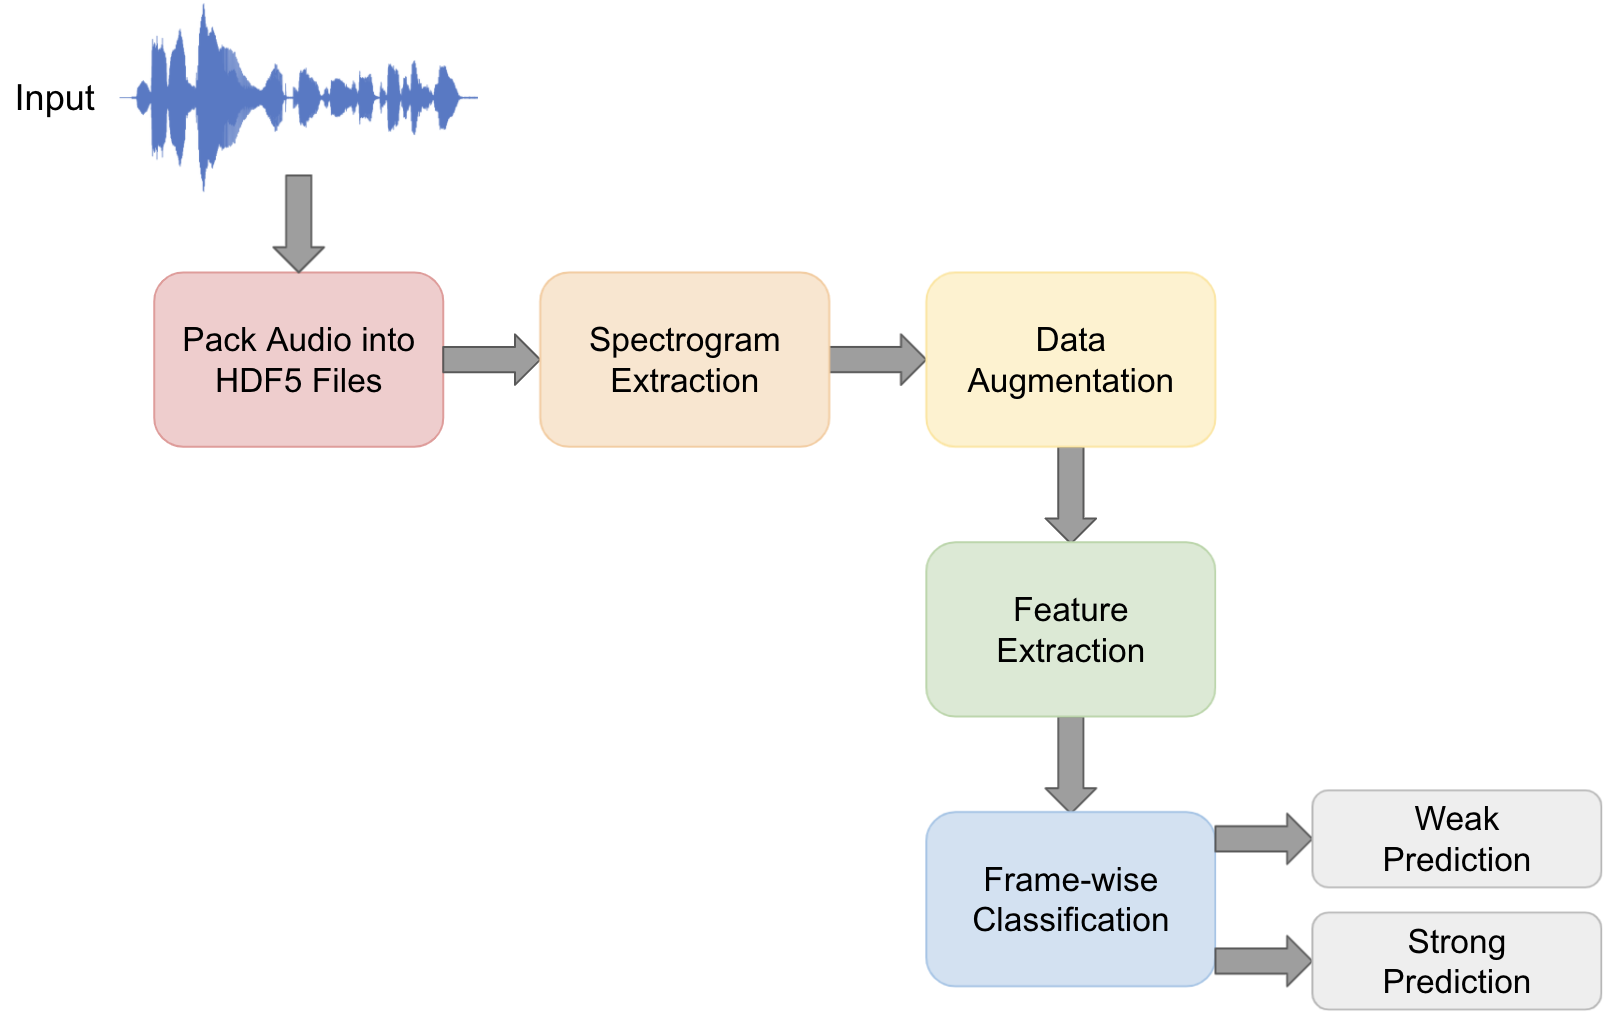
\includegraphics[width=\textwidth]{fig/training-system.png}
    \caption{Overview of training system}
    \label{fig:training-system}
\end{figure}

\subsection{Prediction System}
The prediction system implements the trained system from Section 3.3.1 and analyses audio input that is independent of the audio clips used in the training set and validation set. This system is used to experiment and determine the impact of applying the optimised thresholds, as well as segmenting audio clips before prediction and further processing after prediction. Figure \ref{fig:prediction-system} illustrates the structure of the prediction system.

\begin{figure}[!htb]
    \centering
    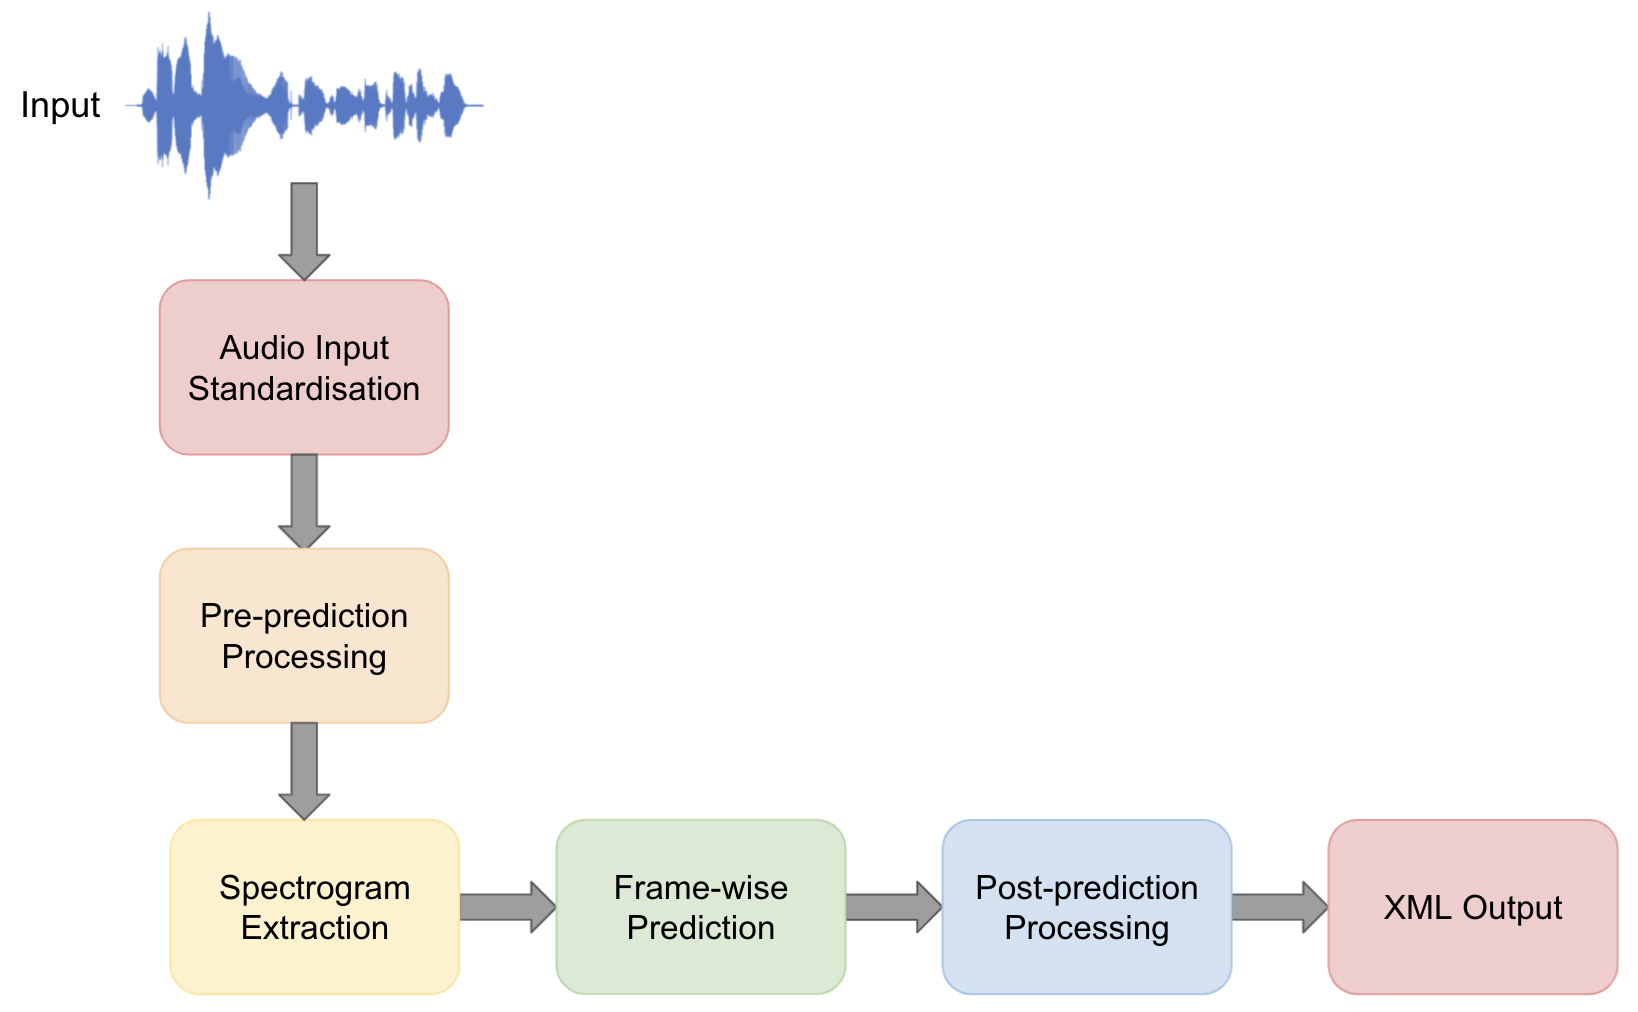
\includegraphics[width=\textwidth]{fig/prediction-system.png}
    \caption{Overview of prediction system}
    \label{fig:prediction-system}
\end{figure}

\section{Training System Specifications}
This section describes the components of the training system.

\subsection{Audio Input Packing}
The raw audio clip files from the dataset, in WAV format, are segmented into strongly-labelled training, weakly-labelled training, validation and testing sets. For each subset of the dataset, the waveforms are packed into a hdf5 file. This is mainly done to speed up training later on. 

\subsection{Spectrogram Extraction}
The process of extracting different spectrograms from the waveforms is specified in this section.

\subsubsection{Log-mel Spectrograms}
The packed waveforms are passed into the model in batches and their spectrogram representations are extracted. Next, the spectrograms are passed through a mel filterbank to generate mel spectrograms. Finally, a logarithmic operation is applied on the mel spectrograms to obtain log-mel spectrograms. This is done enitrely using Torchlibrosa, which uses GPU acceleration to speed up the process.

\subsubsection{Gammatone Spectrograms}
The process of extracting gammatone spectrograms from the packed waveforms is similar to that of extracting log-mel spectrograms, except it is passed through a gamma filterbank instead of a mel filterbank. Additionally, this process is not sped up using GPU. This is due to the unavailability of such a feature in the Torchlibrosa library.

\subsection{Data Augmentation}
For data augmentation, we employed time and frequency masking from SpecAugment \cite{specaugment}, as well as time-shifting \cite{timeshift} and mixup \cite{mixup}. 
For time-shifting, we randomly chose the frame-shift size by sampling from a Gaussian distribution, with a zero mean and a standard deviation of 90. For mixup, we randomly chose the \(\lambda\) value, as mentioned in equations \ref{eqn:mixup-1} and \ref{eqn:mixup-2}, by sampling from a beta distribution with \(\alpha\) = 0.1. Additionally, we experimented with different combinations of these data augmentation techniques, such as SpecAugment with mixup only, and SpecAugment with both time-shift and mixup. 

\subsection{Neural Network Model}
A CNN-based model is used as the feature extractor to extract the high level features from the spectrograms after data augmentation is applied. The output is then fed into a fully connected layer to do frame-wise classification to obtain the presence probabilities of the sound event classes over time steps.  We experimented with CNN-GRU (GRU here refers to a bidirectional GRU), CNN-Transformer and CNN-Conformer models, since they have achieved comparative performances in previous SED tasks \cite{kong2020sound, xu2017convolutional, Miyazaki2020CONFORMERBASEDSE}, as well as varied the number of convolutional layers used in the CNN portion. The CNN portion can be either modelled by a 9-layer or 14-layer CNN, which have shown to perform well on SED tasks \cite{kong2020sound, torchlibrosa}. Additionally, we experimented with transfer learning, using a pre-trained network as our feature extraction model. 

\subsubsection{CNN-Based Models}
The CNN-based model comprises of a CNN to capture local features, and an additional network, either a GRU, Transformer or Conformer, to capture the long-term temporal dependency. To construct the model, we first apply a CNN, either 9-layer or 14-layer, on the spectrogram in order extract the high level features. Next, the feature maps of the last convolutional layer are utilised to obtain embedding vectors along the time axis. The embedding can be denoted as \(x\) and has a shape of the number of time frames by the number of channels. These embeddings are then passed into the network that captures the long-term temporal dependency, which can be either a GRU, Transformer or Conformer, in order to obtain the output features. A fully connected layer with sigmoid activation is applied then on this output to predict the presence probabilities of sound event classes over time steps.

% \subsubsection{CNN-GRU}
% As mentioned in Section 2.5.2, there a few types of CRNNs we can consider to implement to tackle a SED task. For this thesis, we focus on the CNN-GRU since the performance of GRUs are on par with LSTMs, but are computationally more efficient \cite{chung2014empirical}. To construct the CNN-GRU, we first apply a CNN, either 9-layer or 14-layer, on the spectrogram in order extract the high level features. Next, the feature maps of the last convolutional layer are utilised to obtain embedding vectors along the time axis. The embedding can be viewed as \(x\) with a shape of the number of time frames by the number of channels. These embeddings are then passed into the GRU in order to obtain the output features. A fully connected layer with sigmoid activation is applied on this output to predict the presence probabilities of sound event classes over time steps.

% \subsubsection{CNN-Transformer}\\[0.1in]
% %For SED, the input is usually a time-frequency representation such as a log-mel spectrogram. A spectrogram is a low level feature and CNNs have been proposed to apply on the spectrogram representations to extract high level features \cite{cnn-at}. 
% To build the CNN-Transformer system, a CNN, either 9-layer or 14-layer, is applied on the spectrogram representation of an audio clip, followed by a transformer block. Convolutional layers in the CNN are used to extract high level features of the input spectrograms. We use the feature maps of the last convolutional layer to obtain embedding vectors along the time axis, whcih are then fed as input to the transformer. The embedding can be viewed as \(x\) with a shape of the number of time frames by the number of channels. The output of the transformer has a shape of \(T \times d_v\). A fully connected layer followed by a sigmoid non-linearity is applied on this output to predict the presence probabilities of sound classes over time steps. 
% %An aggregation function such as average aggregation can be applied to average out those probabilities along the time domain to obtain the weakly-labelled result. This is an important function as this result is used for training the weakly-labelled train set, which makes up a large portion of the entire train set.

% \subsubsection{CNN-Conformer}\\[0.1in]
% %Similar to the CNN-Transformer, the input is typically a time-frequency representation such as a log-mel spectrogram. 

% Similar to the CNN-GRU and CNN-Transformer, the CNN-Conformer system is constructed by applying a CNN described in Section 2.6.1 on the spectrograms of the audio input. The CNN is used to extract high level features of the input spectrograms. The feature maps of the last convolutional layer are utilised to obtain embedding vectors along the time axis. The embedding can be viewed as x with a shape of the number of time frames by the number of channels. These embeddings are then passed into the conformer block to generate the output features. A fully connected layer with sigmoid activation is applied on this output to predict the presence probabilities of sound classes over the time steps. %Like the CNN-Transformer, aggregation functions such as average aggregation can then be applied to average out those probabilities along the time domain to obtain the weakly-labelled result. This result is used for training the weakly-labelled subset of the train set.

\subsubsection{Transfer Learning}
As discussed in Section 2.5.5, there are two main transfer learning strategies we can apply. In our approach, we only focus on the second strategy, which is to fine-tune the pre-trained model on the project dataset. This involves transferring the weights from a pre-trained CNN, and then fine tuning the network using the new target data. In this thesis, we used the VGGish \cite{vggish} pre-trained model to conduct transfer learning. VGGish is a CNN model from Google that has been pre-trained on the YouTube-8M dataset. The architecture of this network is inspired by the famous VGG \cite{vgg} networks used for image classification. In our experiment, we used VGGish as a feature extractor, fine-tuned on our project dataset, to obtain the output features of an input spectrogram. These output features would later be fed into a classifier, which is a fully connected layer with sigmoid activation to predict the presence probabilities of sound event classes over the time steps.

\subsection{Clip-wise Training}
The clip-wise training method involves feeding entire audio clips as training input, instead of segmenting them beforehand. As such, this method does not explicitly assign tags for each frame \(x_m\). It learns the tags of \(x_m\) implicitly instead from the hidden layer of a neural network. The frame-wise prediction of a frame \(x_m\) can be denoted as \(f(x_m)\). Then, the prediction on an audio clip \(X\) can be obtained by aggregating the frame-wise predictions. This is done to obtain the weakly-labelled result, which is used for training the weakly-labelled subset of the train set. The aggregation can be an average or attention function over the prediction of all frames of each sound event class \(k\). The average function can be defined as:
\begin{equation}
F(X)_k = \sum^M_{m=1}f(x_m)_k .
\end{equation}
% To apply the average function, we include an additional fully-connected layer with sigmoid activation in the network.

To employ the attention function, an additional feed-forward neural network with softmax activation is introduced to infer the temporal locations of each occurring sound event class. In order to preserve the time resolution of the input whole audio spectrogram, we adjust the pooling steps in the CNN-based models by only pooling on the spectral axis while not pooling on the time axis. The feed-forward with sigmoid activation does classification at each frame, while the feed-forward with softmax activation attends to the most important frames for each sound event class. The attention function can be concisely defined as:
\begin{equation}
F(X)_k = \sum^M_{m=1}f(x_m)_k p(x_m)_k ,
\end{equation}
where \(p(x_m) = \frac{exp(w(x_m)_k)}{\sum^M_{j=1}exp(w(x_j)_k)}\), and \(w(\cdot)\) is a linear transformation.\\

As there are two types of data in the development dataset, which are namely the weakly-labelled training set and strongly-labelled training set, each input batch contains a 3 to 1 ratio of the weakly-labelled and strongly-labelled data respectively. We therefore have two different methods of calculating the loss between the predictions and the ground truth for these two types of data.  For the weakly-labelled training set, we calculate the categorical binary loss between the clip-level prediction \(F(X)\) and the weak ground truth label of \(X\) as:
\begin{equation}
E = -\sum^K_{k=1}[y_k\log{F(X)_k} + (1 - y_k)log(1 - F(X)_k)] .
\end{equation}

For the strongly-labelled training set, we calculate the categorical binary loss between the frame-wise prediction \(f(x_m)\) and the strong ground truth of \(X\) as:
\begin{equation}
E = -\sum^M_{m=1} \sum^K_{k=1}[y_k\log{f(x_m)_k} + (1 - y_k)log(1 - f(x_m)_k)],
\end{equation}

where \(y \in \{0, 1\}^K\) represents the tag of each frame, with \(K\) denoting the number of sound event classes. Finally, we sum the weak and strong losses together, which is then used as the main loss function to minimise when training the overall model.

\subsection{Automatic Threshold Optimisation}
In this step, we first optimize the systems and evaluate them based on the metrics that do not depend on the thresholds such as mean average precision (mAP). Next, for a trained system, we optimize the thresholds over a specific metric such as F1-score. To do so, we followed the steps below:

\begin{enumerate}
    \item Initialise thresholds \(\Theta\), where \(\Theta\) consists of the thresholds for each of the sound event classes.
    \item Obtain predictions for each audio clip by applying \(\Theta\).
    \item Initialise loss function J, which is based on negative F1-score. The reason for using such a metric is because minimizing negative F1-score is equivalent to maximising F1 score.
    \item Calculate the gradient of each parameter \(\theta_k\) in \(\Theta\) using the following formula:
    \begin{equation}
    \nabla_\theta J(\Theta) = \frac{J(\Theta + \delta\Theta) - J(\Theta)}{\delta\theta} ,    
    \end{equation}
    \item Apply gradient descent \cite{ruder2016overview} after calculating the numerical gradient of all parameters to obtain optimised thresholds \(\Theta_{opt}\). Gradient descent optimisation can be denoted as:
    \begin{equation}
    \Theta \leftarrow \Theta - \alpha \nabla\Theta J ,
    \end{equation}
    where \(\alpha\) denotes the learning rate.
    The Adam optimiser \cite{kingma2017adam} is then used to optimise J(\(\Theta\)) due to its fast convergence.
\end{enumerate}

% A more concise explanation of the automatic threshold optimisation algorithm is shown in Algorithm 3.1 below.

\section{Prediction System Specification}

\subsection{Audio Input Standardisation}
An audio clip recording of any format can be passed into the system, but those that are not in WAV format will be automatically converted from their original format to WAV. This is done using the FFmpeg package.

\subsection{Pre-Prediction Segmentation and Frame-wise Class Predictions}
The pre-prediction segmentation step involves segmenting the input audio clip into segments of x seconds before passing them into the trained system to obtain the frame-wise class predictions. 
% This pre-prediction processing method has not been used in previous works on SED. 
In this approach, we apply a \(x\) second rolling window with a \(y\) second stride on an audio clip. The values of \(x\) and \(y\) are tuned according to the F1-score of the validation set, which was done using a grid search method \cite{lavalle2004relationship}. We initialised a set of possible rolling window values as \(X\), where \(X\) ranges from 2 to 10, with a step of 0.5, and a set of possible stride values as \(Y\), where \(Y\) ranges from 0.5 to 1.5, with a step of 0.5.\\ 

By applying a rolling window and sending these portioned segments of the audio clip to the trained system to be predicted on individually, some segments may be overlapped. The number of overlaps varies based on the position of the segment on the time axis. For instance, if we apply a 5 second rolling window with a 1 second stride on an audio clip, the maximum number of overlaps a segment can have is 4, while the minimum is 0. An illustration, Figure \ref{fig:overlap}, is shown below to provide a clearer explanation on the varying number of overlaps for each segment in a 14-second long audio clip.

\begin{figure}[!htb]
    \centering
    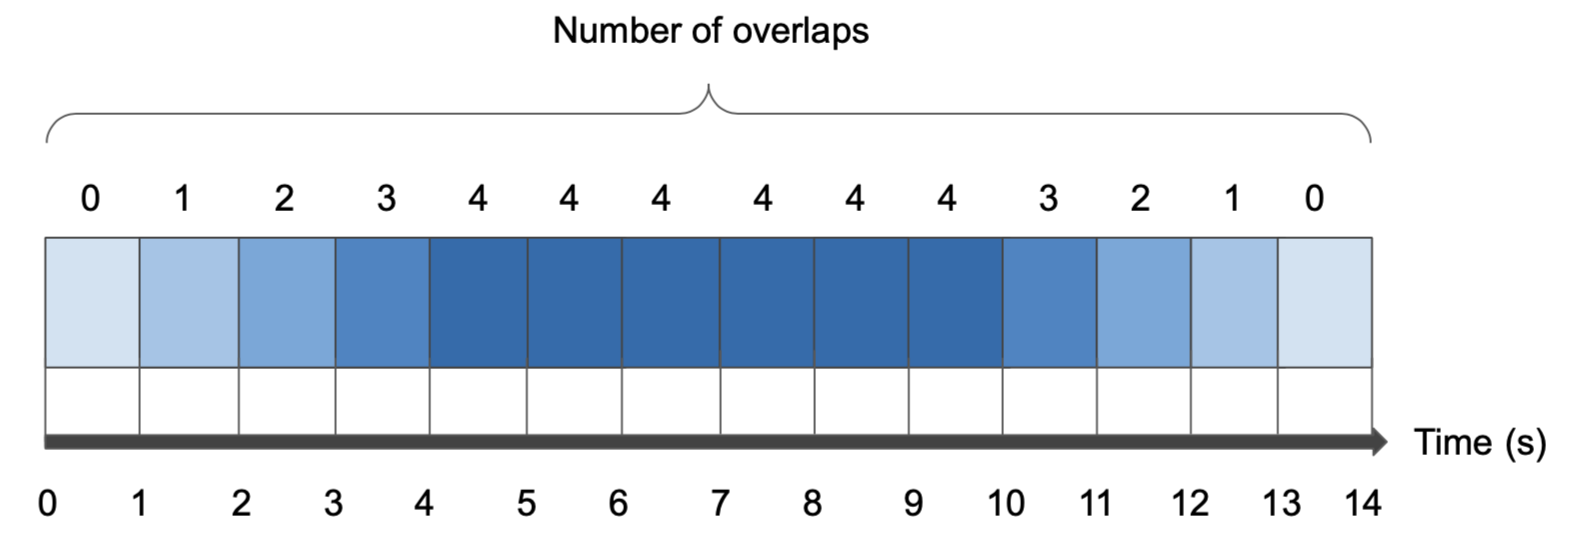
\includegraphics[width=\textwidth]{fig/overlap.png}
    \caption{Example of prediction overlap}
    \label{fig:overlap}
\end{figure}

\subsection{Post-Prediction Processing}
The post-prediction processing step involves manipulating the frame-wise predictions summed across the segments which were overlapped. As shown in Figure 3.3, the number of overlaps differs for each segment as it is dependent on the position of the segment on the time axis. In this thesis, we have proposed two methods of amalgamating the predictions, which is to 1) average the frame-wise predictions or 2) implement a voting scheme.   

\subsubsection{Averaging Frame-wise Predictions}
In this method we first sum the frame-wise predictions together and then average them based on the number of overlaps present in a particular segment. Once the averaged frame-wise predictions are obtained, we apply a set of thresholds, such as the optimised thresholds, over them to determine which sound events are present in which frames. If sequential frames are detected to contain a certain sound event, we determine the onset and offset times of the sound event to correspond to the first and last frames in the sequence, respectively.

\subsubsection{Voting Scheme}
This method involves using a set of thresholds, such as the optimised thresholds, to determine the presence of a sound event. If present, a numerical value of 1 is assigned to the frame for that particular sound event, otherwise 0 is assigned. Next, we sum the binarized frame-wise predictions together and then threshold based on the number of overlaps present in each particular segment. This is done to determine which sound events are present in which frames. Similar to the preceeding method, if sequential frames are detected to contain a certain sound event, we determine the onset and offset times of the sound event to correspond to the first and last frames in the sequence, respectively.

% The post-prediction processing step involves manipulating the frame-wise predictions summed across the segments which were overlapped. In this thesis, we have proposed a method of doing so, which is to average the frame-wise predictions based on the number of overlaps present in a particular segment. As shown in Figure 3.3, the number of overlaps differs for each segment as it is dependent on the position of the segment on the time axis. Once the averaged frame-wise predictions are obtained, we apply a set of thresholds over them to determine which sound events are present in which frames. If sequential frames are detected to contain a certain sound event, we determine the onset and offset times of the sound event to correspond to the first and last frames in the sequence, respectively.

\subsection{Prediction Output Format}
Once we have determined the onset and offset times of the sound events present in an audio clip, we compile them and output them in a XML style format. Figure \ref{fig:xml-output} shows an example of the output of our prediction system.

\begin{figure}[!htb]
    \centering
    \begin{lstlisting}[language=XML]
<AudioDoc name="audio_filename">
    <SoundCaptionList>
        <SoundSegment stime="0.32" duration="9.76">Applause</SoundSegment>
        <SoundSegment stime="0.48" duration="0.96">Cheering</SoundSegment>
        <SoundSegment stime="3.88" duration="5.84">Cheering</SoundSegment>
                                .
                                .
                                .
        <SoundSegment stime="464.32" duration="1.96">Male_speech_man_speaking</SoundSegment>
        <SoundSegment stime="473.16" duration="0.40">Clapping</SoundSegment>
        <SoundSegment stime="473.32" duration="0.68">Male_speech_man_speaking</SoundSegment>
    </SoundCaptionList>
</AudioDoc>
    \end{lstlisting}
    \caption{Prediction system output}
    \label{fig:xml-output}
\end{figure}

\section{Tools and Technologies}
This section summarises the tools and packages used in the development of the SED system.

\subsection{Environment Setup}
Table \ref{tab:env} below provides an overview of the environment setup of this project.

\begin{table}[!htp]
\centering
\begin{tabular}{|c|c|}
\hline
\textbf{Hardware}         & NVIDIA Tesla V100 32 GB \\ \hline
\textbf{Operating System} & Linux                   \\ \hline
\end{tabular}
\caption{\label{tab:env}Environment setup}
\end{table}

\subsection{Language and Libraries}
The SED system was created with a combination of different libraries. Table \ref{tab:tools-libraries} below provides a summary of tools and technologies used in this project. The source code of this project is written entirely in Python.

\begin{table}[!htp]
\centering
\begin{tabular}{|c|c|}
\hline
\textbf{Component}                                                                                                                                                                           & \textbf{Libraries}                                                                                                     \\ \hline
\begin{tabular}[c]{@{}c@{}}Project dataset curation\\ Audio input packing\\ Spectrogram transformation\\ System training\\ Audio input standardisation\\ Performance evaluation\end{tabular} & \begin{tabular}[c]{@{}c@{}}YouTube-DL, FFmpeg\\ HDF5\\ TorchLibrosa, NumPy\\ PyTorch\\ FFmpeg\\ sed\_eval\end{tabular} \\ \hline
\end{tabular}
\caption{\label{tab:tools-libraries}Tools and Libraries used}
\end{table}

\subsubsection{Python}
Python \cite{python} is a programming language predominantly used for this project due to the existing libraries that are useful for developing the SED system. For example, libraries such as PyTorch, which is discussed further in Section 3.6.2.2, is the foundation of our project as we used it to build and train models we experimented with in this thesis. 

\subsubsection{PyTorch}
PyTorch \cite{NEURIPS2019_9015} is a Python package that provides high-level features such as tensor computation with strong GPU acceleration, and deep neural networks built on a tape-based auto-grad system. We used this package to build the models we experimented with in this thesis, as well as speed up training by using a GPU alongside it. 

\subsubsection{FFmpeg}
FFmpeg \cite{tomar2006converting} is a command line program for transcoding multimedia files. It is a very fast video and audio converter that can also collect data from a live audio/video source. It can also convert between arbitrary sample rates and resize video on the fly with a high quality polyphase filter. We used this program to standardise the input audio files to WAV format in the prediction system.

\subsubsection{Librosa}
Librosa \cite{brian_mcfee_2021_4792298} is a Python package for music and audio analysis. It provides the building blocks necessary to create music information retrieval systems. It provides functions to load and resample audio files, and to transform waveforms to different audio feature representations.

\subsubsection{TorchLibrosa}
TorchLibrosa \cite{torchlibrosa} is a PyTorch implementation of some librosa functions to transform raw waveforms to spectrograms with GPU acceleration. It provides almost identical features to the standard librosa functions, with numerical difference less than 1e-5. However, it is limited in its usage as it can only generate log-mel spectrograms as of late.

\subsubsection{YouTube-DL}
YouTube-DL is a command-line program to download audio and videos from YouTube.com and over one thousand other video hosting websites. We used this library to download the corresponding subset of AudioSet audio files from YouTube in order to curate our project dataset.

\subsubsection{sed\textunderscore{eval}}
sed\textunderscore{eval} \cite{sed-eval} is an open source Python toolbox which provides a standardized, and transparent way to evaluate sound event detection systems. This toolbox has been used as the main evaluation function for all the SED DCASE challenges.

\subsubsection{HDF5}
HDF5 \cite{hdf5} is a data software library and file format that is used to manage, process, and store heterogeneous data. It is built for fast I/O processing and storage. We used this library to store our data in order speed up the training and evaluation processes.

%=== END OF PROPOSED APPROACH ===
\newpage
\lhead{Implementation}
\linespread{1.3}
\chapter{Implementation}
This section elaborates on the development process and components of the SED training system.

% \section{Training System}
% This subsection elaborates on the components of the training system.

\section{Spectrogram Extraction}
We experimented with log-mel spectrograms and gammatone spectrograms as input features. To begin with, all the audio clips are converted to monophonic and resampled to 8k Hz or 16k Hz, depending on the quality of the development dataset used. The following describes the conversion details for the log-mel spectrograms.\\ 

If the 8k Hz dataset is used, Short Time Fourier Transform (STFT) with a Hanning window of 256 samples and hop size of  80 samples is used to extract a spectrogram which produces 100 frames per second. Next, 64 mel filter banks are applied on the spectrogram, followed by logarithmic operation to compute the log-mel spectrogram. The number 64 is selected as it can be evenly divided by a power of 2 in the down-sampling layers of CNNs. The mel filter banks have a lower cut-off frequency of 12 Hz and a higher cut-off frequency of 3.5 kHz to avoid aliasing caused by resampling.\\

If the 16k Hz dataset is used, STFT with a Hanning window of 512 samples and a hop size of 160 samples is used to extract a spectrogram. Similarly, 64 mel filter banks are applied on the spectrogram, followed by logarithmic operation to generate a log-mel spectrogram. The mel filter banks have a lower cut-off frequency of 25 Hz and a higher cut-off frequency of 7 kHz.
\

\section{Neural Network Model}
As mentioned in Section 3.4.4, feature extraction is done with a CNN-based model. Then, a time-distributed fully connected layer with sigmoid non-linearity is applied to predict the presence probability of sound events of each time frame. We experimented with a variety of models, such as CNN-GRU, CNN-Transformer, and CNN-Conformer. Within such models, we also experimented with the number of layers in the CNN component, specifically 9 layers and 14 layers. 

\subsection{9-layer vs 14-layer CNN}
The 9-layer CNN consists of 4 convolutional blocks, where each convolutional block comprises of 2 convolutional layers with kernel sizes of 3 × 3, with each convolutional layer followed by batch normalization [40] and ReLU non-linearity [50]. The convolutional block consists of 64, 128, 256 and 512 feature maps, respectively. Each convolutional block is followed by a 2 × 2 average pooling to extract high level features. No residual connections is applied in our CNNs as gradient vanishing is not an issue with 8 convolutional layers. Finally, the frequency axis of the output from the last convolutional layer is averaged out. A concise description of the 9-layer CNN can be found in Table \ref{tab:cnn-9}, whereby the number following @ represents the number of feature maps. The second column shows the number of batch size (bs), feature maps, frames and frequency bins. The third column states the number of parameters in each component. 
% Then, the time-distributed fully connected layer with sigmoid non-linearity is applied to predict the presence probability of sound events of each time frame.\\

\begin{table}[!htp]
\centering
\begin{tabular}{|c|c|c|}
\hline
\textbf{Layers}                                                       & \textbf{Output Size} & \textbf{Number of Parameters} \\ \hline
Input                                                                 & bs x 1 x 640 x 64    & -                             \\ \hline
\begin{tabular}[c]{@{}c@{}}(3 x 3 @ 64 \\ BN, ReLU) x 2\end{tabular}  & bs x 64 x 640 x 64   & 37,696                        \\ \hline
2 x 2 avg. pooling                                                    & bs x 64 x 320 x 32   & -                             \\ \hline
\begin{tabular}[c]{@{}c@{}}(3 x 3 @ 128 \\ BN, ReLU) x 2\end{tabular} & bs x 128 x 320 x 32  & 221,696                       \\ \hline
2 x 2 avg. pooling                                                    & bs x 128 x 160 x 16  & -                             \\ \hline
\begin{tabular}[c]{@{}c@{}}(3 x 3 @ 256 \\ BN, ReLU) x 2\end{tabular} & bs x 256 x 160 x 16  & 885,760                       \\ \hline
2 x 2 avg. pooling                                                    & bs x 256 x 80 x 8    & -                             \\ \hline
\begin{tabular}[c]{@{}c@{}}(3 x 3 @ 512 \\ BN, ReLU) x 2\end{tabular} & bs x 512 x 80 x 8    & 3,540,992                     \\ \hline
Avg. frequency bins                                                   & bs x 512 x 80 x 1    & -                             \\ \hline
\end{tabular}
\caption{\label{tab:cnn-9}9-layer CNN architecture}
\end{table}

The 14-layer CNN consists of 6 convolutional blocks, in which each convolutional block contains 2 convolutional layers, each having 3 × 3 kernel sizes. Batch normalisation and ReLU are applied after each convolutional layer. Additionally, a 2 × 2 average pooling is also applied after each convolutional layer to extract high level features. The 6 convolution blocks consist of 64, 128, 256, 512, 1024 and 2048 feature maps respectively. A concise description of the 14-layer CNN can be found in Table \ref{tab:cnn-14}.

\begin{table}[!htp]
\centering
\begin{tabular}{|c|c|c|}
\hline
\textbf{Layers}                                                        & \textbf{Output Size} & \textbf{Number of Parameters} \\ \hline
Input                                                                  & bs x 1 x 640 x 64    & -                             \\ \hline
\begin{tabular}[c]{@{}c@{}}(3 x 3 @ 64 \\ BN, ReLU) x 2\end{tabular}   & bs x 64 x 640 x 64   & 37,696                        \\ \hline
2 x 2 avg. pooling                                                     & bs x 64 x 320 x 32   & -                             \\ \hline
\begin{tabular}[c]{@{}c@{}}(3 x 3 @ 128 \\ BN, ReLU) x 2\end{tabular}  & bs x 128 x 320 x 32  & 221,696                       \\ \hline
2 x 2 avg. pooling                                                     & bs x 128 x 160 x 16  & -                             \\ \hline
\begin{tabular}[c]{@{}c@{}}(3 x 3 @ 256 \\ BN, ReLU) x 2\end{tabular}  & bs x 256 x 160 x 16  & 885,760                       \\ \hline
2 x 2 avg. pooling                                                     & bs x 256 x 80 x 8    & -                             \\ \hline
\begin{tabular}[c]{@{}c@{}}(3 x 3 @ 512 \\ BN, ReLU) x 2\end{tabular}  & bs x 512 x 80 x 8    & 3,540,992                     \\ \hline
2 x 2 avg. pooling                                                     & bs x 512 x 40 x 4    & -                             \\ \hline
\begin{tabular}[c]{@{}c@{}}(3 x 3 @ 1024 \\ BN, ReLU) x 2\end{tabular} & bs x 1024 x 40 x 4   & 14,159,872                              \\ \hline
2 x 2 avg. pooling                                                     & bs x 1024 x 20 x 2   & -                             \\ \hline
\begin{tabular}[c]{@{}c@{}}(3 x 3 @ 2048 \\ BN, ReLU) x 2\end{tabular} & bs x 2048 x 20 x 2   & 56,631,296                              \\ \hline
Avg. frequency bins                                                    & bs x 2048 x 20 x 1   & -                             \\ \hline
\end{tabular}
\caption{\label{tab:cnn-14}14-layer CNN architecture}
\end{table}

\subsection{CNN-GRU}
The CNN-GRU is a CNN, either 9 or 14 layers, with a bi-directional GRU. The output features of the CNN are passed into the bi-directional GRU. The bi-directional GRU consists of 1 recurrent layer, with 256 features in the hidden state.

\subsection{CNN-Transformer}
The CNN-Transformer is a CNN, either 9 or 14 layers, with a transformer block. The output features of the CNN are passed into the transformer. The transformer consists of 8 attention heads and 512 attention units. Additionally, it contains a dropout layer with a dropout rate of 0.1. 

\subsection{CNN-Conformer}
The CNN-Conformer is a CNN, either 9 or 14 layers, with a conformer block. The output features of the CNN are passed into the conformer. The conformer consists of 4 attention heads and 144 attention units. The conformer block was stacked 4 times and the kernel size of the depthwise convolution is 7. Additionally, it contains a dropout layer with a dropout rate of 0.1.

\subsection {Transfer Learning}
The VGGish pre-trained model used to conduct transfer learning consists of a series of convolution and activation layers, followed by a max pooling layer. This network contains 17 layers in total, and can be fine-tuned during model training. We removed the last three layers of the original VGGish model and used the output of the last convolutional layer as our input data for the frame-wise classifier. A summary of the architecture of VGGish can be found in Table \ref{tab:vggish}.

\begin{table}[!htp]
\centering
\begin{tabular}{|
>{\columncolor[HTML]{FFFFFF}}c |
>{\columncolor[HTML]{FFFFFF}}c |
>{\columncolor[HTML]{FFFFFF}}c |}
\hline
{\color[HTML]{333333} \textbf{Layers}}                            & \textbf{Output Size} & \textbf{Number of Parameters} \\ \hline
Input                                                             & bs x 1 x 640 x 64    & -                             \\ \hline
\begin{tabular}[c]{@{}c@{}}3 x 3 @ 64 \\ ReLU\end{tabular}        & bs x 64 x 640 x 64   & 640                           \\ \hline
2 x 2 max pooling                                                 & bs x 64 x 320 x 32   & -                             \\ \hline
\begin{tabular}[c]{@{}c@{}}3 x 3 @ 128 \\ ReLU\end{tabular}       & bs x 128 x 320 x 32  & 73,856                        \\ \hline
2 x 2 max pooling                                                 & bs x 128 x 160 x 16  & -                             \\ \hline
\begin{tabular}[c]{@{}c@{}}(3 x 3 @ 256 \\ ReLU) x 2\end{tabular} & bs x 256 x 160 x 16  & 885,248                       \\ \hline
2 x 2 max pooling                                                 & bs x 256 x 80 x 8    & -                             \\ \hline
\begin{tabular}[c]{@{}c@{}}(3 x 3 @ 512 \\ ReLU) x 2\end{tabular} & bs x 512 x 80 x 8    & 3,539,968                     \\ \hline
2 x 2 max pooling                                                 & bs x 512 x 40 x 4    & -                             \\ \hline
\end{tabular}
\caption{\label{tab:vggish}VGGish architecture}
\end{table}

\section{Clip-wise Training}
As mentioned in Section 3.4.5, the aggregation methods we experimented with included an average or attention function over the predictions of all segments of each sound class. The average function uses a simple mean function from PyTorch to obtain the clip-wise output. The attention function uses an additional feed-forward neural network with softmax activation to attend to the most important frames for each class and infer the temporal locations of each occuring sound event class. The number of output feature maps is equivalent to the number of sound event classes present in the development dataset, which is 25.\\

% The attention-based method is done using a feed-forward CNN, which consists of two convolutional layers. The first layer, with sigmoid activation, does classification at each frame, while the second layer, with softmax activation, attends to the most important frames for each class. The number of output feature maps is equivalent to the number of sound event classes present in the development dataset, which is 25.\\

During training, the Adam optimizer \cite{kingma2017adam} with a learning rate of 0.001 is applied. The training is stopped at 50,000 iterations and the performance of the model is evaluated every 1,000 iterations on the strongly-labelled validation set, using the mean average precision (mAP) metric and error rate. mAP is used here as it does not depend on the threshold value. Only the best-performing model, which has the highest mAP score and lowest error rate, is saved. 

\section{Automatic Threshold Optimisation}
The threshold of each sound event class was optimised using gradient descent iteratively. This process ran for 70 epochs and the output of each epoch was evaluated based on the F1-score. Only the thresholds from the epoch with the highest F1-score are saved. 

%=== END OF PROPOSED APPROACH ===
\newpage
\lhead{Results and Discussion}
%=== Results_and_Discussion ===
%=== (Actual work done and contribution, including literature survey) ===

\chapter{Experiments and Results}

\section{Experiments}
We experimented with a number of SED systems, using different variations of the spectrogram representation, data augmentation technique, model type,  post-prediction method and threshold type. All the experiments were done on the higher quality dataset, with audio clips of 16k Hz. We evaluated these SED systems on the test set of the project dataset mentioned in Section 3.1. The test set consists of 747 audio clip files, each around 10 seconds long.\\ 

We conducted the experiments in a sequential manner, that is, we first experimented with the audio features, with other variables constant. Once the best audio feature type is determined, we move on to experiment with the data augmentation techniques, followed by model types, then threshold types, and finally the post-prediction processing methods. Ideally, we would have experimented with all the different combinations of the variables to determine the best-performing system. However, we were unable to do so due to time and resource constraints.\\ 
% Hence, we performed the experiments sequentially instead.\\

In order to make the experiments more comprehensive, we also evaluated the best-performing SED system with the lower quality dataset, with 8k Hz audio clips, mentioned in Section 3.1.1. In this evaluation, our SED system is trained from scratch using the lower quality 8k Hz dataset, and then evaluated on the corresponding test set. This is done to determine how the SED system would perform with data we would more likely obtain in real-life scenarios.\\

Next, we evaluated the best-performing SED systems, based on the 16k Hz project dataset, on the DCASE 2017 Task 4 dataset in order to determine whether our proposed systems are comparable with state-of-the-art systems as well. In this evaluation, our SED system is trained from scratch again using the DCASE 2017 training set, which consists of 51,172 weakly-labelled audio clips, validated using the validation set, consisting of 488 clips and then evaluated on the test set, which contains 1,103 clips. Each audio clip is around 10 seconds long.\\

Finally, we evaluated our SED system on longer audio clips in order to observe the effects of our proposed pre-prediction and post-prediction processing method on them. However, as it is costly and very time consuming to annotate audio clips with strong labels, we only evaluated two 1-minute long audio clips, which is 6 times longer than the 10 second long audio clips in our project dataset. These two audio clips, which are independent of the audio clips in the development dataset, were downloaded from YouTube and manually-labelled ourselves.

\section{Evaluation Metric}
The evaluation metric used in this thesis follows the metric used in the DCASE 2017 Task 4 challenge \cite{DCASE2017}, which is segment-based evaluation with error rate and F1-score. The segment-based evaluation is done in a fixed time grid, in which segments of one second length are used to compare the groundtruth and system output. In each segment k, we count the number of each of the following values:
\begin{itemize}

\item{true positives (TP) - active events as indicated by both the ground truth and system output;}
\item{false positives (FP) - active events as indicated by the system output but inactive according to the ground truth;}
\item{false negatives (FN) - inactive events as indicated by the system output but active according to the ground truth;} 
\item{substitutions (S) - occur when the system output wrongly indicates an event as active; one substitution is equivalent to one FP and one FN, which means that the system did not detect the correct event (FN for the correct class) but detected something (FP for another class);}
\item{insertions (I) - number of FPs after subtracting the substitutions;}
\item{deletions (D) - number of FNs after subtracting the substitutions;}
\item{reference events (N) - number of sound events in the ground truth.}

\end{itemize}

\subsection{Error Rate}
The computation of the error rate ER follows the formula described in \cite{Poliner2007}. It is calculated over all the test data using the total number of insertions I, deletions D and substitutions S, and is formulated as follows:
\begin{equation}
ER = \sum{S(k)} + \sum{D(k)} + \sum{I(k)}\sum{N(k)}.    
\end{equation}

\subsection{F1-Score}
The F1-score F can be described as the harmonic mean of the precision P and recall R scores. It is calculated over all the test data based on the total number of false positives FPs, false negatives FNs, and true positives TPs, and is formulated as follows:
\begin{equation}
F = \frac{2(P \times R)}{P + R},
\end{equation}

where \(P = \frac{\sum{TP(k)}}{\sum{TP(k)} + \sum{FP(k)}}\) and \(R = \frac{\sum{TP(k)}}{\sum{TP(k)} + \sum{FN(k)}}\).

\section{Results}

This section summarises the results of the experiments conducted for this project.

\subsection{Results for Different Audio Feature Types}
The data augmentation technique, model type, threshold type, and pre-prediction and post-prediction processing method are constant and set to SpecAugment with mixup, 9-layer CNN with GRU and attention aggregation, non-optimised thresholds, and none, respectively. The results of the experiment with the varied audio feature types are summarised in Table \ref{tab:spec-res}.

\begin{table}[!htp]
\centering
\begin{tabular}{|c|c|c|c|c|}
\hline
\textbf{Spectrogram Representation}                         & \textbf{Error Rate}                                   & \textbf{F1-Score}                                     & \textbf{Precision}                                    & \textbf{Recall}                                       \\ \hline
\begin{tabular}[c]{@{}c@{}}Log-mel\\ Gammatone\end{tabular} & \begin{tabular}[c]{@{}c@{}}\textbf{0.555}\\ 0.569\end{tabular} & \begin{tabular}[c]{@{}c@{}}\textbf{0.624}\\ 0.605\end{tabular} & \begin{tabular}[c]{@{}c@{}}0.718\\ \textbf{0.732}\end{tabular} & \begin{tabular}[c]{@{}c@{}}\textbf{0.552}\\ 0.516\end{tabular} \\ \hline
\end{tabular}
\caption{\label{tab:spec-res}Comparison of spectrogram representations}
\end{table}

% \begin{table}[!htp]
%     \scriptsize
%     \centering
%     \begin{tabularx}{\textwidth}{llrlRRRRRR}
% \toprule
% &Spectrogram Representation& 
%         Segment-based Error Rate &
%                 Segment-based F1-Score &
%                         Precision&    Recall&    SAR&    STOI &  ESTOI & WER\\ \midrule
% \multirow{9}{*}{\makecell[cl]{\rotatebox{90}{Raw}}}
% &\multirow{1}{*}{\makecell[cl]{Log-mel}} &
% \multirow{1}{*}{0.555}&
% 0.624 &0.718    &0.552\\
% \cline{2-10}
% &\multirow{1}{*}{Gammatone} &
% \multirow{1}{*}{0.569}&
% 0.605 &0.732    &0.516\\
% \cline{2-10}

% \bottomrule
%     \end{tabularx}
%     \caption[Performance summary for two-source separation]{Performance summary for two-source separation\\}
%     \label{tab:summary2}
% \end{table}

\subsection{Results for Different Data Augmentation Techniques}
From the preceding experiment, we have determined that using the log-mel spectrogram representation produced a better performing system. As such, it is used as the audio feature in the following experiments. The model type, post-prediction processing method, and threshold type are the same as those in the preceding experiment. The results of the experiment with the varied data augmentation techniques are summarised in Table \ref{tab:data-aug-res}.\\

\begin{table}[!htp]
\centering
\resizebox{\textwidth}{!}{\begin{tabular}{|c|c|c|c|c|}
\hline
\textbf{Data Augmentation Technique}                                                                                                                                                          & \textbf{Error Rate}                                                                                   & \textbf{F1-Score}                                                                                     & \textbf{Precision}                                                                                    & \textbf{Recall}                                                                                       \\ \hline
\begin{tabular}[c]{@{}c@{}}None\\ SpecAugment\\ Mixup\\ Time-shift\\ SpecAugment \& Mixup\\ SpecAugment \& Time-shift\\ Mixup \& Time-shift\\ SpecAugment \& Mixup \& Time-shift\end{tabular} & \begin{tabular}[c]{@{}c@{}}0.599\\ 0.592\\ 0.567\\ 0.614\\ \textbf{0.555}\\ 0.599\\ 0.606\\ 0.583\end{tabular} & \begin{tabular}[c]{@{}c@{}}0.589\\ 0.600\\ 0.611\\ 0.563\\ \textbf{0.624}\\ 0.596\\ 0.569\\ 0.598\end{tabular} & \begin{tabular}[c]{@{}c@{}}0.674\\ 0.660\\ \textbf{0.740}\\ 0.698\\ 0.718\\ 0.670\\ 0.730\\ 0.727\end{tabular} & \begin{tabular}[c]{@{}c@{}}0.523\\ \textbf{0.551}\\ 0.521\\ 0.472\\ 0.552\\ 0.536\\ 0.466\\ 0.507\end{tabular} \\ \hline
\end{tabular}}
\caption{\label{tab:data-aug-res}Comparison of data augmentation techniques}
\end{table}

\subsection{Results for Different Model Types}
From the preceding experiments, we have determined that the log-mel spectrogram representation and SpecAugment with mixup produced a better performing system. As such, they are used as the audio feature and data augmentation technique, respectively, in the following experiments. The threshold type and post-prediction processing method are the same as those in the preceeding experiment. The results of the experiment with the varied model types are summarised in Table \ref{tab:model-res}.

\begin{table}[!htp]
\centering
\resizebox{\textwidth}{!}{\begin{tabular}{|c|c|c|c|c|c|}
\hline
\textbf{Model}                                                                                                                                                                                                                                                                                                         & \textbf{Error Rate}                                                                                                           & \textbf{F1-Score}                                                                                                             & \textbf{Precision}                                                                                                            & \textbf{Recall}                                                                                                               & \textbf{\begin{tabular}[c]{@{}c@{}}Model Size\\ (\# parameters)\end{tabular}}                                                                                                \\ \hline
\begin{tabular}[c]{@{}c@{}}CNN-9-GRU-Attention\\ CNN-9-GRU-Average\\ CNN-14-GRU-Attention\\ CNN-9-Transformer-Attention\\ CNN-9-Transformer-Average\\ CNN-14-Transformer-Attention\\ CNN-9-Conformer-Attention\\ CNN-9-Conformer-Average\\ CNN-14-Conformer-Attention\\ VGGish-Attention\\ VGGish-Average\end{tabular} & \begin{tabular}[c]{@{}c@{}}0.555\\ 0.604\\ 0.590\\ \textbf{0.552}\\ 0.633\\ 0.559\\ 0.560\\ 0.638\\ 0.584\\ 0.681\\ 0.676\end{tabular} & \begin{tabular}[c]{@{}c@{}}0.624\\ 0.591\\ 0.585\\ \textbf{0.628}\\ 0.544\\ 0.617\\ 0.620\\ 0.555\\ 0.596\\ 0.506\\ 0.520\end{tabular} & \begin{tabular}[c]{@{}c@{}}0.718\\ 0.664\\ 0.714\\ 0.712\\ 0.696\\ \textbf{0.732}\\ 0.666\\ 0.627\\ 0.682\\ 0.672\\ 0.618\end{tabular} & \begin{tabular}[c]{@{}c@{}}0.552\\ 0.532\\ 0.495\\ 0.562\\ 0.447\\ 0.533\\ \textbf{0.580}\\ 0.497\\ 0.530\\ 0.406\\ 0.448\end{tabular} & \begin{tabular}[c]{@{}c@{}}5,894,692\\ 5,881,817\\ 94,466,596\\ 5,763,620\\ 5,750,745\\ 79,781,924\\ 6,280,493\\ 6,276,818\\ 77,295,917\\ 5,708,260\\ 5,695,385\end{tabular} \\ \hline
\end{tabular}}
\caption{\label{tab:model-res}Comparison of model types}
\end{table}

\subsection{Results for Applying Optimised Thresholds}
From the preceding experiment, we determined that the 9-layer CNN with Transformer, the 9-layer CNN with Conformer, and 9-layer CNN with GRU models, all with attention aggregation applied, produced the better performing models. We tested these three models in the following experiments, while keeping the audio feature and data augmentation technique used the same as those in the preceding experiment. No pre-prediction or post-prediction processing methods are applied. The results of the experiment of applying the optimised thresholds are summarised in Table \ref{tab:thres-res}.

\begin{table}[!htp]
\centering
\begin{tabular}{|c|c|c|c|c|c|}
\hline
\textbf{Model}                                                            & \textbf{Threshold Type}                                           & \textbf{Error Rate}                                   & \textbf{F1-Score}                                     & \textbf{Precision}                                    & \textbf{Recall}                                       \\ \hline
\begin{tabular}[c]{@{}c@{}}CNN-9\\ -GRU\\ -Attention\end{tabular}         & \begin{tabular}[c]{@{}c@{}}Non-optimised\\ Optimised\end{tabular} & \begin{tabular}[c]{@{}c@{}}0.555\\ 0.601\end{tabular} & \begin{tabular}[c]{@{}c@{}}0.624\\ 0.635\end{tabular} & \begin{tabular}[c]{@{}c@{}}\textbf{0.718}\\ 0.619\end{tabular} & \begin{tabular}[c]{@{}c@{}}0.552\\ \textbf{0.651}\end{tabular} \\ \hline
\begin{tabular}[c]{@{}c@{}}CNN-9\\ -Transformer\\ -Attention\end{tabular} & \begin{tabular}[c]{@{}c@{}}Non-optimised\\ Optimised\end{tabular} & \begin{tabular}[c]{@{}c@{}}\textbf{0.552}\\ 0.561\end{tabular} & \begin{tabular}[c]{@{}c@{}}0.628\\ \textbf{0.648}\end{tabular} & \begin{tabular}[c]{@{}c@{}}0.712\\ 0.650\end{tabular} & \begin{tabular}[c]{@{}c@{}}0.562\\ 0.646\end{tabular} \\ \hline
\begin{tabular}[c]{@{}c@{}}CNN-9\\ -Conformer\\ -Attention\end{tabular}   & \begin{tabular}[c]{@{}c@{}}Non-optimised\\ Optimised\end{tabular} & \begin{tabular}[c]{@{}c@{}}0.560\\ 0.591\end{tabular} & \begin{tabular}[c]{@{}c@{}}0.620\\ 0.629\end{tabular} & \begin{tabular}[c]{@{}c@{}}0.675\\ 0.617\end{tabular} & \begin{tabular}[c]{@{}c@{}}0.599\\ 0.642\end{tabular} \\ \hline
\end{tabular}
\caption{\label{tab:thres-res}Comparison of threshold types}
\end{table}

\subsection{Results for Post-Prediction Processing Methods}
From the preceding experiment, we can observe that applying optimised thresholds does not consistently improve the performance of the system across all the evaluation metrics. As such, we continued experimenting with both non-optimised and optimised thresholds in the following experiments, while using the same audio feature, data augmentation technique, and model types as the experiment in Section 5.3.4. The results of the experiments with the three best-performing model types, implementing the different post-prediction processing methods are summarised in Table \ref{tab:process-res}.

\begin{table}[!htp]
\centering
\resizebox{\textwidth}{!}{\begin{tabular}{|c|c|c|c|c|c|c|c|}
\hline
\textbf{Model}                                                                             & \textbf{\begin{tabular}[c]{@{}c@{}}Processing \\ Type\end{tabular}} & \textbf{Threshold Type}                                           & \textbf{Error Rate}                                                             & \textbf{F1-Score}                                                               & \textbf{Precision}                                                              & \textbf{Recall}                                                                 & \textbf{\begin{tabular}[c]{@{}c@{}}Process Time\\ (Seconds)\end{tabular}} \\ \hline
\multirow{3}{*}{\begin{tabular}[c]{@{}c@{}}CNN-9\\ -GRU\\ -Attention\end{tabular}}         & None                                                                & \begin{tabular}[c]{@{}c@{}}Non-optimised\\ Optimised\end{tabular} & \begin{tabular}[c]{@{}c@{}}0.555\\ 0.601\end{tabular}                           & \begin{tabular}[c]{@{}c@{}}0.624\\ 0.635\end{tabular}                           & \begin{tabular}[c]{@{}c@{}}0.718\\ 0.619\end{tabular}                           & \begin{tabular}[c]{@{}c@{}}0.552\\ 0.651\end{tabular}                           & 25.124                                                                    \\ \cline{2-8} 
                                                                                           & \begin{tabular}[c]{@{}c@{}}Frame-wise \\ averaging\end{tabular}     & \begin{tabular}[c]{@{}c@{}}Non-optimised\\ Optimised\end{tabular} & \begin{tabular}[c]{@{}c@{}}0.557\\ 0.574\end{tabular}                           & \begin{tabular}[c]{@{}c@{}}0.618\\ 0.639\end{tabular}                           & \begin{tabular}[c]{@{}c@{}}\textbf{0.749}\\ 0.645\end{tabular} & \begin{tabular}[c]{@{}c@{}}0.525\\ 0.634\end{tabular}                           & 35.931                                                                    \\ \cline{2-8} 
                                                                                           & Voting                                                              & \begin{tabular}[c]{@{}c@{}}Non-optimised\\ Optimised\end{tabular} & \begin{tabular}[c]{@{}c@{}}0.658\\ 0.711\end{tabular}                           & \begin{tabular}[c]{@{}c@{}}0.572\\ 0.560\end{tabular}                           & \begin{tabular}[c]{@{}c@{}}0.624\\ 0.574\end{tabular}                           & \begin{tabular}[c]{@{}c@{}}0.528\\ 0.547\end{tabular}                           & 43.302                                                                    \\ \hline
\multirow{3}{*}{\begin{tabular}[c]{@{}c@{}}CNN-9\\ -Transformer\\ -Attention\end{tabular}} & None                                                                & \begin{tabular}[c]{@{}c@{}}Non-optimised\\ Optimised\end{tabular} & \begin{tabular}[c]{@{}c@{}}0.552\\ 0.561\end{tabular}                           & \begin{tabular}[c]{@{}c@{}}0.628\\ 0.648\end{tabular}                           & \begin{tabular}[c]{@{}c@{}}0.712\\ 0.650\end{tabular}                           & \begin{tabular}[c]{@{}c@{}}0.562\\ 0.646\end{tabular}                           & 25.947                                                                    \\ \cline{2-8} 
                                                                                           & \begin{tabular}[c]{@{}c@{}}Frame-wise \\ averaging\end{tabular}     & \begin{tabular}[c]{@{}c@{}}Non-optimised\\ Optimised\end{tabular} & \begin{tabular}[c]{@{}c@{}}\textbf{0.549}\\ 0.550\end{tabular} & \begin{tabular}[c]{@{}c@{}}0.622\\ \textbf{0.648}\end{tabular} & \begin{tabular}[c]{@{}c@{}}0.747\\ 0.667\end{tabular}                           & \begin{tabular}[c]{@{}c@{}}0.533\\ 0.628\end{tabular}                           & 33.682                                                                    \\ \cline{2-8} 
                                                                                           & Voting                                                              & \begin{tabular}[c]{@{}c@{}}Non-optimised\\ Optimised\end{tabular} & \begin{tabular}[c]{@{}c@{}}0.562\\ 0.675\end{tabular}                           & \begin{tabular}[c]{@{}c@{}}0.643\\ 0.628\end{tabular}                           & \begin{tabular}[c]{@{}c@{}}0.663\\ 0.569\end{tabular}                           & \begin{tabular}[c]{@{}c@{}}0.623\\ \textbf{0.700}\end{tabular} & 38.923                                                                    \\ \hline
\multirow{3}{*}{\begin{tabular}[c]{@{}c@{}}CNN-9\\ -Conformer\\ -Attention\end{tabular}}   & None                                                                & \begin{tabular}[c]{@{}c@{}}Non-optimised\\ Optimised\end{tabular} & \begin{tabular}[c]{@{}c@{}}0.560\\ 0.591\end{tabular}                           & \begin{tabular}[c]{@{}c@{}}0.620\\ 0.629\end{tabular}                           & \begin{tabular}[c]{@{}c@{}}0.666\\ 0.617\end{tabular}                           & \begin{tabular}[c]{@{}c@{}}0.580\\ 0.642\end{tabular}                           & 18.227                                                                    \\ \cline{2-8} 
                                                                                           & \begin{tabular}[c]{@{}c@{}}Frame-wise \\ averaging\end{tabular}     & \begin{tabular}[c]{@{}c@{}}Non-optimised\\ Optimised\end{tabular} & \begin{tabular}[c]{@{}c@{}}0.560\\ 0.563\end{tabular}                           & \begin{tabular}[c]{@{}c@{}}0.611\\ 0.635\end{tabular}                           & \begin{tabular}[c]{@{}c@{}}0.699\\ 0.646\end{tabular}                           & \begin{tabular}[c]{@{}c@{}}0.611\\ 0.624\end{tabular}                           & 24.645                                                                    \\ \cline{2-8} 
                                                                                           & Voting                                                              & \begin{tabular}[c]{@{}c@{}}Non-optimised\\ Optimised\end{tabular} & \begin{tabular}[c]{@{}c@{}}0.662\\ 0.683\end{tabular}                           & \begin{tabular}[c]{@{}c@{}}0.562\\ 0.557\end{tabular}                           & \begin{tabular}[c]{@{}c@{}}0.615\\ 0.600\end{tabular}                           & \begin{tabular}[c]{@{}c@{}}0.518\\ 0.520\end{tabular}                           & 31.836                                                                    \\ \hline
\end{tabular}}
\caption{\label{tab:process-res}Comparison of processing methods}
\end{table}

\subsection{Results of SED System Trained on Lower Audio Quality Dataset}
From the preceeding experiments, we have determined that using log-mel spectrogram representation, SpecAugment with mixup, optimised thresholds and averaging frame-wise predictions method in post-processing produced the best-performing systems. We re-trained these systems, which were based on the 16k dataset, on the 8k dataset. The results of the experiment with the system trained on the lower audio quality dataset are summarised in Table \ref{tab:quality-res}.

\begin{table}[!htp]
\centering
\resizebox{\textwidth}{!}{\begin{tabular}{|c|c|c|c|c|c|}
\hline
\textbf{Model}                                                            & \textbf{Audio Quality}                           & \textbf{Error Rate}                                   & \textbf{F1-Score}                                     & \textbf{Precision}                                    & \textbf{Recall}                                       \\ \hline
\begin{tabular}[c]{@{}c@{}}CNN-9\\ -GRU\\ -Attention\end{tabular}         & \begin{tabular}[c]{@{}c@{}}8k\\ 16k\end{tabular} & \begin{tabular}[c]{@{}c@{}}0.629\\ 0.574\end{tabular} & \begin{tabular}[c]{@{}c@{}}0.618\\ 0.639\end{tabular} & \begin{tabular}[c]{@{}c@{}}0.607\\ 0.645\end{tabular} & \begin{tabular}[c]{@{}c@{}}0.629\\ 0.634\end{tabular} \\ \hline
\begin{tabular}[c]{@{}c@{}}CNN-9\\ -Transformer\\ -Attention\end{tabular} & \begin{tabular}[c]{@{}c@{}}8k\\ 16k\end{tabular} & \begin{tabular}[c]{@{}c@{}}0.574\\ 0.550\end{tabular} & \begin{tabular}[c]{@{}c@{}}0.638\\ 0.648\end{tabular} & \begin{tabular}[c]{@{}c@{}}0.642\\ 0.667\end{tabular} & \begin{tabular}[c]{@{}c@{}}0.627\\ 0.628\end{tabular} \\ \hline
\begin{tabular}[c]{@{}c@{}}CNN-9\\ -Conformer\\ -Attention\end{tabular}   & \begin{tabular}[c]{@{}c@{}}8k\\ 16k\end{tabular} & \begin{tabular}[c]{@{}c@{}}0.570\\ 0.563\end{tabular} & \begin{tabular}[c]{@{}c@{}}0.630\\ 0.635\end{tabular} & \begin{tabular}[c]{@{}c@{}}0.645\\ 0.646\end{tabular} & \begin{tabular}[c]{@{}c@{}}0.617\\ 0.624\end{tabular} \\ \hline
\end{tabular}}
\caption{\label{tab:quality-res}Comparison of dataset quality}
\end{table}

\subsection{Results of SED System Trained on DCASE 2017 Dataset}
In order to have a state-of-the-art baseline for comparison, we re-trained the different systems we experimented with in the previous sections with the DCASE 2017 dataset \cite{DCASE2017}. The results of our experiments are summarised in Table \ref{tab:dcase2017-res}.

\begin{table}[!htp]
\centering
\resizebox{\textwidth}{!}{\begin{tabular}{|c|c|c|c|c|c|c|}
\hline
\textbf{Model}                                                                             & \textbf{\begin{tabular}[c]{@{}c@{}}Processing \\ Type\end{tabular}} & \textbf{Threshold Type}                                           & \textbf{Error Rate}                                   & \textbf{F1-Score}                                     & \textbf{Precision}                                    & \textbf{Recall}                                       \\ \hline
State-of-the-art                                                                           & -                                                                   & -                                                                 & 0.680                                                 & 0.584                                                 & 0.625                                                     & 0.548                                                     \\ \hline
\multirow{2}{*}{\begin{tabular}[c]{@{}c@{}}CNN-9\\ -GRU\\ -Attention\end{tabular}}         & None                                                                & \begin{tabular}[c]{@{}c@{}}Non-optimised\\ Optimised\end{tabular} & \begin{tabular}[c]{@{}c@{}}0.659\\ 0.650\end{tabular} & \begin{tabular}[c]{@{}c@{}}0.578\\ \textbf{0.594}\end{tabular} & \begin{tabular}[c]{@{}c@{}}0.603\\ \textbf{0.633}\end{tabular} & \begin{tabular}[c]{@{}c@{}}0.555\\ 0.559\end{tabular} \\ \cline{2-7} 
                                                                                           & \begin{tabular}[c]{@{}c@{}}Frame-wise \\ averaging\end{tabular}     & \begin{tabular}[c]{@{}c@{}}Non-optimised\\ Optimised\end{tabular} & \begin{tabular}[c]{@{}c@{}}0.665\\ \textbf{0.643}\end{tabular} & \begin{tabular}[c]{@{}c@{}}0.569\\ 0.585\end{tabular} & \begin{tabular}[c]{@{}c@{}}0.607\\ 0.619\end{tabular} & \begin{tabular}[c]{@{}c@{}}0.536\\ \textbf{0.651}\end{tabular} \\ \hline
\multirow{2}{*}{\begin{tabular}[c]{@{}c@{}}CNN-9\\ -Transformer\\ -Attention\end{tabular}} & None                                                                & \begin{tabular}[c]{@{}c@{}}Non-optimised\\ Optimised\end{tabular} & \begin{tabular}[c]{@{}c@{}}0.738\\ 0.703\end{tabular} & \begin{tabular}[c]{@{}c@{}}0.549\\ 0.565\end{tabular} & \begin{tabular}[c]{@{}c@{}}0.545\\ 0.592\end{tabular} & \begin{tabular}[c]{@{}c@{}}0.553\\ 0.540\end{tabular} \\ \cline{2-7} 
                                                                                           & \begin{tabular}[c]{@{}c@{}}Frame-wise \\ averaging\end{tabular}     & \begin{tabular}[c]{@{}c@{}}Non-optimised\\ Optimised\end{tabular} & \begin{tabular}[c]{@{}c@{}}0.728\\ 0.696\end{tabular} & \begin{tabular}[c]{@{}c@{}}0.548\\ 0.547\end{tabular} & \begin{tabular}[c]{@{}c@{}}0.555\\ 0.595\end{tabular} & \begin{tabular}[c]{@{}c@{}}0.541\\ 0.505\end{tabular} \\ \hline
\multirow{2}{*}{\begin{tabular}[c]{@{}c@{}}CNN-9\\ -Conformer\\ -Attention\end{tabular}}   & None                                                                & \begin{tabular}[c]{@{}c@{}}Non-optimised\\ Optimised\end{tabular} & \begin{tabular}[c]{@{}c@{}}0.689\\ 0.695\end{tabular} & \begin{tabular}[c]{@{}c@{}}0.557\\ 0.559\end{tabular} & \begin{tabular}[c]{@{}c@{}}0.585\\ 0.585\end{tabular} & \begin{tabular}[c]{@{}c@{}}0.531\\ 0.536\end{tabular} \\ \cline{2-7} 
                                                                                           & \begin{tabular}[c]{@{}c@{}}Frame-wise \\ averaging\end{tabular}     & \begin{tabular}[c]{@{}c@{}}Non-optimised\\ Optimised\end{tabular} & \begin{tabular}[c]{@{}c@{}}0.689\\ 0.692\end{tabular} & \begin{tabular}[c]{@{}c@{}}0.550\\ 0.552\end{tabular} & \begin{tabular}[c]{@{}c@{}}0.585\\ 0.592\end{tabular} & \begin{tabular}[c]{@{}c@{}}0.519\\ 0.517\end{tabular} \\ \hline
\end{tabular}}
\caption{\label{tab:dcase2017-res}Comparison of systems trained on DCASE 2017 dataset}
\end{table}

\subsection{Results on Longer Audio Clips}
In order to demonstrate the impact of our proposed averaging frame-wise predictions method on longer audio clips, we evaluated two longer audio clips, which we manually labelled, using one of our best-performing models, the 9-layer CNN with GRU and attention aggregation. We used the same audio feature and data augmentation  technique as the previous experiments, and set the threshold type to optimised. For the baseline, we analysed the audio clips in non-overlapping 3-second segments. For the averaging frame-wise prediction method, we analysed the audio clips in 3-second segments with a 0.5-second stride. We evaluated each audio clip against their respective groundtruth based on error rate and F1-score, and recorded the results in Table \ref{tab:long-res}.

\begin{table}[!htb]
\centering
\resizebox{\textwidth}{!}{\begin{tabular}{|c|c|c|c|c|c|}
\hline
\textbf{Audio Clip} & \textbf{\begin{tabular}[c]{@{}c@{}}Processing \\ Type\end{tabular}} & \textbf{Error Rate} & \textbf{F1-Score} & \textbf{Precision} & \textbf{Recall} \\ \hline
\multirow{2}{*}{A}  & None                                                                & 0.427               & 0.720             & 0.794              & 0.659           \\ \cline{2-6} 
                    & Frame-wise averaging                                                & \textbf{0.256}               & \textbf{0.880}             & \textbf{0.794}              & \textbf{0.988}           \\ \hline
\multirow{2}{*}{B}  & None                                                                & 0.244               & 0.867             & 0.818              & 0.923           \\ \cline{2-6} 
                    & Frame-wise averaging                                                & \textbf{0.205}               & \textbf{0.886}             & \textbf{0.831}              & \textbf{0.949}           \\ \hline
\end{tabular}}
\caption{\label{tab:long-res}Comparison of processing methods for longer audio clips}
\end{table}

\section{Discussion}
This section discusses the results obtained from the experiments conducted for this project.

\subsection{Discussion for Audio Feature Type}
From Table \ref{tab:spec-res}, we can observe that the system trained with the log-mel spectrograms performed better than the one trained with gammatone spectrograms, achieving better results for both error rate and F1-score. Furthermore, the generation of the log-mel spectrograms can be significantly sped up by PyTorch through GPU acceleration, using TorchLibrosa, while the gammatone spectrograms cannot. As such, there is a significantly greater incentive to use the log-mel spectrogram representations for training. 

\subsection{Discussion for Data Augmentation Techniques}
From Table \ref{tab:data-aug-res}, we can observe the performances of the system without data augmentation applied, and with various methods of data augmentation applied. These results show that when applied individually, SpecAugment and mixup did improve the performance of the system, while time-shift did not. Although not statistically significant, a combination of SpecAugment and time-shift, and a combination of SpecAugment, mixup and time-shift did manage to improve the performance of the system. However, a combination of SpecAugment and mixup yielded the most statistically significant improvement from the original system where no data augmentation technique applied. Both the error rate and F1-score improved from 0.599 and 0.589 to 0.555 and 0.624, respectively.

\subsection{Discussion for Model Types}
From Table \ref{tab:model-res}, we can observe that the 9-layer CNN with Transformer and attention aggregation model performed the best. Additionally, it is also one of the smallest models we experimented with. In fact, it is the smallest model among the top 3 best-performing models, which includes the 9-layer CNN with GRU and attention aggregation, and the 9-layer CNN with Conformer and attention aggregation. Hence, this makes the 9-layer CNN with Transformer and attention the most ideal model to use, out of all the models, as it is both the best-performing, and one of the smaller and more portable models.\\

In general, using a 14-layer CNN as opposed to a 9-layer CNN increases the model size exponentially, by around 13 times, and also seems to worsen the performance of the models. This is because adding more layers may have caused the data to overfit during training. Additionally, the models which employed attention aggregation consistently performed significantly better than the ones which used average aggregation. This suggests that attention plays an important role in weakly-lablled training for SED tasks. Furthermore, for our particular task at hand, transfer learning does not seem to be helpful. In fact, the model which applied transfer learning with the VGGish pre-trained network performed the worst out of all the model types we experimented with.

\subsection{Discussion for Automatic Threshold Optimisation}
Based on Table \ref{tab:thres-res}, we can observe that using the optimised thresholds does consistently improve the performance of the systems, in terms of the F1-score. 
% Specifically, it significantly improves the recall score. 
This can be attributed to the fact that different sound event classes have different thresholds to achieve their optimal F1-score. This can be observed from their precision-recall curves under various thresholds, as shown in Figure \ref{fig:precision-recall-curves}. As depicted, some sound event classes such as 'Gunshot, gunfire' have high precision and high recall at a variety of thresholds. On the other hand, the precision drops significantly as recall increases for some sound event classes, such as 'Run'.\\

\begin{figure}[!htb]
    \centering
    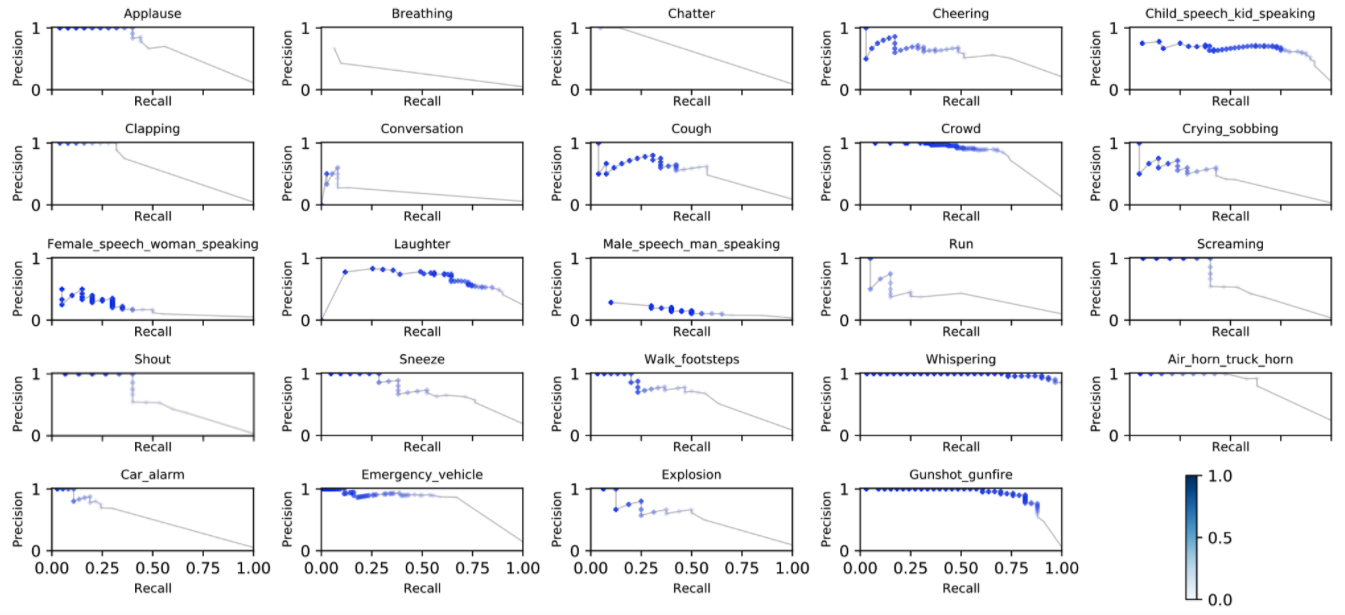
\includegraphics[width=\textwidth]{fig/precision-recall-curves.png}
    \caption{Precision-recall curves of different sound event classes at different thresholds with the CNN-Transformer-Attention system}
    \label{fig:precision-recall-curves}
\end{figure}

However, applying the optimised thresholds also consistently worsens the error rate slightly. Since the performance improvement is not consistent across all the evaluation metrics, we continue experimenting with both optimised and non-optimised thresholds in the subsequent experiments.

\subsection{Discussion for Post-Prediction Processing Methods}
From Table \ref{tab:process-res}, we can observe that averaging the frame-wise predictions in post-processing, combined with applying the optimised thresholds did improve the performance of the system. Specifically, both error rate and F1-score improved consistently across all the three model types, as compared to the previous experiment where we only applied the optimised thresholds. On the other hand, the voting scheme method generally performed worse when compared to the averaging frame-wise predictions method, which may have been attributed to its more stringent threshold scheme. Notably, applying the voting scheme method alone, as opposed to combining it with the optimised thresholds, yielded better results in comparison.\\ 

Although applying the averaging frame-wise predictions method does yield a better performing system, it should be noted that doing so increases the processing time. The total audio duration for the clips in the test set amounts to 7,470 seconds (2 hours 4 minutes 30 seconds). Taking the CNN-9-Transformer-Attention model as an example, without this additional step of averaging the frame-wise prediction, the total processing time for the test set is 25.95 seconds. When we average the frame-wise predictions, the total processing time increases to 33.68 seconds, up 29.8\% from the original. This increase in processing time may be attributed to the averaging frame-wise predictions method processing certain segments of an audio clip several times, while not doing so enables each segment of the audio clip to be processed just once. Since processing time is an important factor to consider as it affects user experience, and may be critical for certain usages, one should determine whether the averaging frame-wise prediction method is worth implementing based on their individual goals.

% From  Table  5-5  in  Section  5.2.5,  we  can  observe  that  averaging  the  frame-wise  predictions  in  post-processing,  combined  with  applying  the  optimisedthresholds did improve the performance of the system. Specifically, both errorrate and F1-score improved consistently across all the three model types,  ascompared  to  the  previous  experiment  where  we  only  applied  the  optimisedthresholds.  However, it should be noted that there is an increase in processingtime  when  the  averaging  frame-wise  predictions  method  is  used.   The  totalaudio duration for the clips in the test set amounts to 7470 seconds (2 hours4 minutes 30 seconds). Taking the CNN-9-Transformer-Attention model as anexample, without this additional step of averaging the frame-wise prediction, the total processing time for the test set is 25.95 seconds. When we average theframe-wise predictions in post-processing, the total processing time increasesto  33.68  seconds,  which  is  an  increase  of  29.8 \%  from  the  original.    Thereason for this increase in processing time is because the averaging frame-wisepredictions method processes certain segments of an audio clip several times,while not doing so enables each segment of the audio clip to be processed justonce. Since the processing time is an important factor to take into considerationas it affects the user experience, and may be critical for certain usages of thissystem,  one  should  determine  whether  the  averaging  frame-wise  predictionmethod is worth implementing based on their individual goals.

\subsection{Discussion for Performance on Lower Audio Quality Dataset}
As observed in Table \ref{tab:quality-res}, the performance of the system worsened across all the evaluation metric scores for the 8k dataset. This is as expected since the 8k dataset has a lower audio quality, compared to the 16k dataset, and has additional noise introduced for it to better mimic audio clips the system would receive as input in real-life situations. Despite the poorer results, the performance of the system trained on the 8k dataset is still comparable to that of the system trained on the 16k dataset, with only a slight increase in error rate and a slight decrease in F1-score across all three model types we tested. Specifically, the error rate increased by an average of 5.06\% and the F1-score decreased by an average of 1.87\%. As such, our system is suitable for use in real-life scenarios.

\subsection{Discussion for Performance on DCASE 2017 Dataset}
Based on Table \ref{tab:dcase2017-res}, we can observe that our trained system, namely the CNN-9-GRU-Attention model variations, managed to perform better than the state-of-the-art system \cite{kong2020sound} for the DCASE 2017 Task 4 challenge, in terms of both error rate and F1-score. However, there is a slight difference in the effect of applying frame-wise averaging, when compared to the systems trained on our project dataset. Although applying frame-wise averaging in post-prediction processing does improve the error rate consistently, it does not necessarily improve the F1-score, due to the increased false positive predictions. Since error rate is used as the main metric for evaluating and ranking systems in the DCASE 2017 Task 4 challenge, applying frame-wise averaging still works to our advantage regardless.

\subsection{Discussion for Performance on Longer Audio Clips}
As observed in Table \ref{tab:long-res}, the system which utilised the averaging frame-wise predictions post-processing method performed better than the baseline system which did not, for both of the audio clips. To better understand the reason behind this, a visual analysis for prediction results of one of the audio clips, A, alongside its groundtruth for comparison, is provided in Figure \ref{fig:audio_clip_1_result}.\\

In Figure \ref{fig:audio_clip_1_result}, at around the 20 second mark for instance, we can observe that both the baseline system and the system utilising our proposed method managed to successfully detect the presence of the 'Explosion' sound event. However, the baseline system detected a shorter duration of around 1 second, while the system utilising our proposed method detected a longer duration of around 3 second, which is more similar to that in the groundtruth, in comparison. As mentioned in Section 2.7, this discrepancy in the results is attributed to the fact that the 'Explosion' sound event is broken apart and not analysed as a whole in the baseline system, while the system utilising our proposed method is able to cover all the bases and analyse all the segment partitions with a 0.5-second stride, and finally average out the predictions to return a more optimal result.\\

\begin{figure}[!htb]
    \centering
    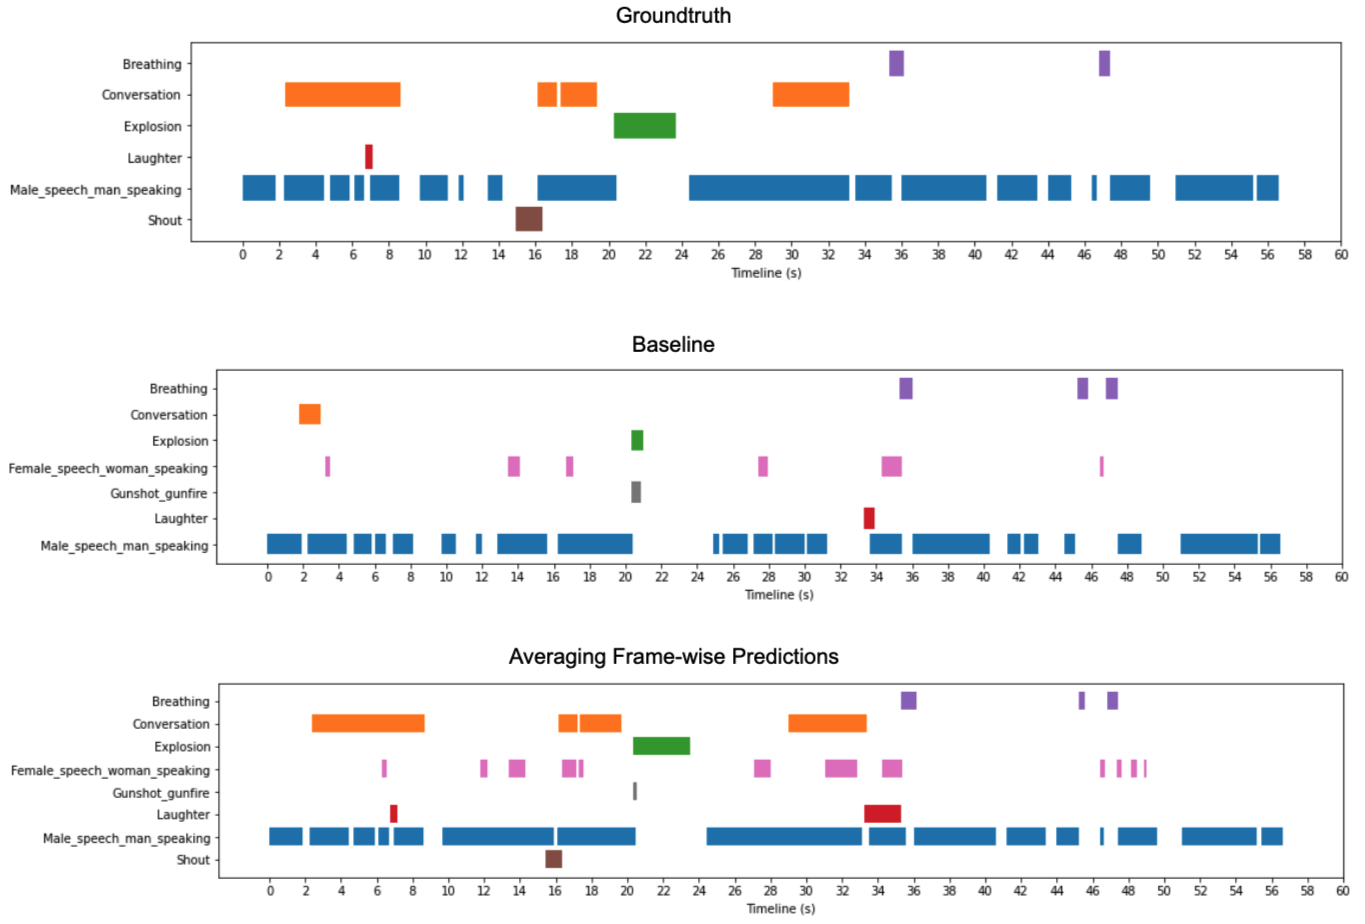
\includegraphics[width=\textwidth]{fig/audio_clip_1_result.png}
    \caption{Prediction results of audio clip A}
    \label{fig:audio_clip_1_result}
\end{figure}

\FloatBarrier %stopping float objects like images 


%=== END OF RESULTS AND DISCUSSION ===
\newpage

\lhead{Conclusion and Future Work}
%=== Conclusion and Recommendations ===

\chapter{Conclusion and Future Work}

\section{Conclusion}
In this thesis, we experimented with different audio feature types, SED model structures and data augmentation techniques, as well as proposed a pre-prediction and post-prediction processing method. From our experiments, we managed to successfully develop a well-performing SED system for our novel dataset. We found that using the log-mel spectrogram representation, SpecAugment and mixup, CNN-9-Transformer-Attention model, optimised thresholds and averaging frame-wise predictions method in post-processing, produced the best-performing system, in terms of both error rate and F1-score. In fact, the incorporation of our proposed averaging frame-wise prediction method consistently improved the system, proving especially useful for longer audio clips.\\

Additionally, by imparting the knowledge we learnt from our experiments with our novel project dataset, we managed to improve from the previous state-of-the-art model for the DCASE 2017 Task 4 Challenge \cite{kong2020sound}. We found that using the log-mel spectrogram representation, SpecAugment with mixup and time-shift, CNN-9-GRU-Attention model, optimised thresholds and averaging frame-wise predictions method in post-processing, produced the best performing system, in terms of error rate. Specifically, we improved the error rate from 0.680, as reported in the previous state-the-art-system \cite{kong2020sound}, to 0.643.

\section{Future Work}
This section discusses the direction of the future work of this thesis.

\subsection{Experiment Comprehensiveness}
Due to the extensiveness of the variables of the system, some variable combinations were not fully examined. In future work, we would like to experiment with all the different combinations of the components of the SED system as this may yield a different outcome to our current best performing system determined from the sequential experimentation technique. Additionally, we would also like to explore the possibility of using other audio feature types, such as constant Q-transform (CQT), and data augmentation techniques, such as pitch change and speed change.

\subsection{Dataset Expansion}
Although one of the objectives of this thesis is to develop a system with a limited amount of strongly-labelled training data, another possible approach we could explore to develop a well-performing SED system would be to generate more strongly-labelled data for training, which would tackle the root of this problem. This can possibly be done by developing a synthetic strongly-labelled dataset using audio clips from FSD50K, with the help of Scaper \cite{scaper2017}. FSD50K \cite{fonseca2020fsd50k} is a publicly available dataset which contains more than 51,000 audio clips that were manually labelled using 200 classes extracted from the AudioSet Ontology \cite{audioset}. In fact, the DCASE 2019 and DCASE 2020 \cite{DCASE2019} challenges on SED both used synthetic clips generated with Scaper, which employed audio clips from FSD50K as foreground sounds, in their strongly-labelled dataset.

%=== END OF CONCLUSION ===
\newpage

\lhead{Bibliography}
\addcontentsline{toc}{chapter}{Bibliography} % see https://tex.stackexchange.com/questions/119719/add-an-item-in-the-table-of-contents
\printbibliography[title={Bibliography}]

%==== ENDING PART ===
  \clearpage
  \pagenumbering{arabic}%
  \renewcommand{\thepage}{R-\arabic{page}}
\lhead{}
%\rhead{References}
%\printbibliography[title={References}]

%=================================
% \newpage
% \appendix
% % \renewcommand{\chapname}{Appendix}
% \pretocmd{\chapter}{%
%   \clearpage
%   \pagenumbering{arabic}%
%   \renewcommand*{\thepage}{\thechapter-\arabic{page}}%
% }{}{}
% % \rhead{Appendix}
% %\lhead{Source Information}
% %=== APPENDIX TABLES ===

\chapter{Appendix}

% \subsection*{Table A-1}

% Table \ref{tab:sourceinfo} shows the speaker initials (ID), sex, dialect region number (DR), and the sentences used for each of the sources. Sentences that are trimmed are denoted with asterisks. 

% \begin{table}[!htp]
%     \footnotesize\centering
%     \begin{tabularx}{\textwidth}{clccLLLL}
% \toprule
% Source & Speaker ID & Sex & DR & Sentences\\
% \midrule
% 1 & JWT0 & M & 1 & SI1291& SI751& SI1381*\\
% 2 & AEM0 & F & 2 & SA1& SA2& SI762& SI1392*\\
% 3 & SLS0 & F & 3 & SI1056& SI1686& SI2316\\
% 4 & BAS0 & F & 4 & SI1387& SI1472& SI2066*\\
% 5 & DWH0 & M & 5 & SI1168& SI1925& SX35\\
% 6 & JRK0 & M & 6 & SI1662& SI2130& SI880& SX160*\\
% \bottomrule
% \end{tabularx}
%     \caption[Speaker information for the evaluation sources]{Speaker information for the evaluation sources\\
%     \footnotesize{M - male; F - female. DR1 - New England; DR2 - Northern; DR3 - North Midland; DR4 - South Midland; DR5 - Southern; DR6 - New York City.}}
%     \label{tab:sourceinfo}
% \end{table}

% \subsection*{Table A-2}

% \begin{table}[!htp]
%     \footnotesize\centering
%     \begin{tabularx}{\textwidth}{cL}
% \toprule
% Source & Transcript\\
% \midrule
% 1 & they should live in modest circumstances avoiding all conspicuous consumption serve in frankfurter buns or as a meat dish but briefly the topping \\
% 2 & 
% she had your dark suit in greasy wash water all year
% don't ask me to carry an oily rag like that
% fill small hole in bowl with clay 
% assume for\\
% 3 & can thermonuclear war be set off by accident it latches when you close it so stay as long as you like Davy Mathews it's disgusting the way you're always eating\\
% 4 & several factors contributed to this change she greeted her husband's colleagues with smiling politeness offering nothing He saw a pint-sized man\\
% 5 & it takes a great deal of sophisticated thought to get the impact of this fact so what's this all about help celebrate your brother's success\\
% 6 & did anyone see my cab See you in about an hour the revolution now under way in materials handling makes this much easier as co-authors we presented our new book\\
% \bottomrule
% \end{tabularx}
%     \caption{Transcript of the evaluation sources}
%     \label{tab:transcript}
% \end{table}
% \newpage %ADD NEW PAGE

% \FloatBarrier

% \subsection{Log-mel Spectrogram Computation}

% The steps for computing log-mel spectrograms are as follows:
% \begin{enumerate}
% \item{Sample the input with Hann windows of \(x\) size, making hops of \(y\) size each time to sample the next window. The values of \(x\) and \(y\) are pre-defined.}
% \item{Map each window from time domain to frequency domain by using the Fast Fourier Transform (FFT) algorithm.}
% \item{Generate a mel scale by taking the entire frequency spectrum, and separating it into \(z\) bins evenly spaced frequencies. The mel scale values are calculated as follows:
% \begin{equation}
%     m = 2595 log_{10}(1 + \frac{f}{100})
% \end{equation}}
% \item{Generate the spectrograms by decomposing the magnitude of the signal into its components, corresponding to the frequencies in the Mel scale, for each window. }
% \item{Apply the logarithmic conversion of the powers at each of the mel scale frequencies.}
% \end{enumerate}

\subsection{Gammatone Spectrogram Computation}
% The steps for computing gammatone spectrograms are as follows:

% \begin{enumerate}
% \item{Sample the input with Hann windows of \(x\) size, making hops of size \(y\) each time to sample the next window. The values of \(x\) and \(y\) are pre-defined.}
% \item{Compute the Discrete Fourier Transform (DFT) for each window \(a^t\):
% \begin{equation}
% A^t_k = \sum^{n−1}_{m=0}a^t_m exp(−2{\pi}i\frac{mk}{n}), \quad k = 0, . . . , n - 1.
% \end{equation}

% Since the input windows are real-valued, the output of the DFT is Hermetian symmetric. Thus, the negative-frequency terms are redundant and can be discarded. The first bin \(A^t_0\) contains the zero-frequency term of the signal and is also discarded. We are then left with \(\frac{n}{2}\) points \(A^t = [A^t_1, A^t_2, ..., A^t_\frac{n}{2}]^T\) for each window.
% \item{The square of the absolute value of each window component is then calculated. The resulting vectors are stacked to establish the power spectrogram A:
% \begin{equation}
% A = [|A^1|^2, |A^2|^2,  ..., |A^t|^2]
% \end{equation}}
% \item{Each bin \(|A^i|^2\) of the power spectrogram is then weighted according to what the magnitude gain of a gammatone filter of the same center frequency would have been for the frequency corresponding to the DFT bin. This can be expressed by the matrix multiplication \(G = W A\). W is computed by transforming the impulse response of m gammatone filters evenly spaced on the ERB scale using an n-point DFT.
% \begin{equation} W = 
% \begin{bmatrix}
% |DFT{g_{f1}(t)|^2\\
% |DFT{g_{f2}(t)|^2\\
% \vdots\\
% |DFT{g_{fm}(t)|^2
% \end{bmatrix}
% \end{equation}}
% \item{Apply the logarithmic conversion of the powers at each of the frequencies.}
% \end{enumerate}

% \subsection{CNN Specifications}
% A standard CNN comprises of convolution layers, pooling layers and fully connected layers. 
% % The input to each convolutional layer is a tensor with a shape (N, C, W, H), where N represents the number of input samples, C is the number of channels, W is the width and H is the height. 
% Each convolutional layer contains a set of learnable kernels, and its output is a tensor known as a feature map. These kernels are able to learn the local time-frequency patterns in the spectrogram extracted from an audio clip. In audio processing, the low level features \cite{thickstun2017learning} can be the raw wave-forms or spectrograms. The high level features are then extracted by the convolutional layers from these low level features. Following recent CNN architecures, batch normalization \cite{ioffe2015batch} is then applied after the convolutional layers to stabilise and increase the speed of training. After each batch normalization, non-linear activation functions, such as ReLU \cite{relu}, are then applied. For SED tasks, pooling layers are also applied along both time and frequency axes. Finally, the output of the last convolutional layer is fed as input to a time-distributed fully connected layer in order to predict the presence probability of sound events along the time axis. 
% %Finally, the predicted probabilities are aggregated over the time axis to obtain the clip-wise sound event presence probability. The aggregation can be, for example, maximum or average operations over the time axis. 

% \subsection{Transformer Specifications}
% A typical transformer may comprise of several encoder and decoder layers. When an input is fed into a transformer, it is transformed into a high level embedding by the encode, which can then be transformed to an output by the decoder. In SED tasks, only the encoder is required, and each encoder is made up several encoder layers. 
% % For each encoder layer, the input is denoted as a tensor \(x\) of shape \(T \times C\), where \(T\) and \(C\) represent the number of time steps and channels, respectively. These symbols follow those used in \cite{vaswani2017attention}. 
% The encoder layer contains a query transform matrix \(W^Q\), a key transform matrix \(W^K\) and a value transform matrix \(W^V\). The matrices \(W^Q\) and \(W^K\) have a shape of \(C × d_k\), and \(W^V\) has a shape of \(C \times d_v\), where \(C\) represents the number of channels, and \(d_k\) and \(d_v\) are integers. Then the query \(Q\),  key \(K\) and value \(V\) can be obtained by:

% \begin{align}
% Q = xW^Q\\
% K = xW^K\\
% V = xW^V 
% \end{align}

% The query Q and key K have a shape of \(T \times d_k\), and the value \(V\) has a shape of \(T \times d_v\), where \(T\) refers to the number of time steps. The output of an encoder layer can be written as: 

% \begin{equation}
% \label{eqn:trans-4}
% h = softmax(\frac{QK^T}{\sqrt{d_k}})V ,
% \end{equation}

% where the output \(h\) has a shape of \(T \times H\). 
% % Equation \ref{eqn:trans-4} computes the dot product of the query with all keys, then divides each product by \(\sqrt{d_k}\), and finally applies a softmax function to obtain the weights on the values V \cite{vaswani2017attention}. 
% In equation \ref{eqn:trans-4}, the division of the square root of \(d_k\) is a normalization term \cite{vaswani2017attention}, and the inner product of \(Q\) and \(K^T\) has a shape of \(T \times T\), which represents the feature correlation of different time steps. The softmax function transforms the correlation value to probabilities along the time steps, which indicate how much the value \(V\) in a time step should be attended to.\\

\subsection{Conformer Specifications}
% The conformer block is made up of three modules, namely a feed-forward module, a multi-head self-attention module, and a convolution module. The feed-forward module comprises of a layer-normalization layer, a linear layer with a Swish activation function \cite{ramachandran2017searching}, which expands the dimensions of the input by four times, and finally another linear layer, which projects the dimensions back to those of the original input. The multi-head self-attention module contains a layer-normalization and multi-head self-attention with relative positional embedding, as used in Transformer-XL \cite{dai-etal-2019-transformer}. The convolution module is made up of a layer normalization layer, a point-wise convolution layer with a gated linear unit (GLU) activation function \cite{dauphin2017language}, and a 1-D depth-wise convolution layer, which is then followed by a batch normalization layer, Swish activation, and finally a point-wise convolution layer. The relation between the input \(X\) and output \(Y\) of the conformer block can thus be modelled as follows:

% \begin{align}
% X˜ = X + \frac{1}{2}FFN(X),\\
% X` = X˜ + MHSA(X˜),\\
% X`` = X` + Conv(X),\\
% Y = LayerNorm(X`` + \frac{1}{2}FFN(X``)),  
% \end{align}

% where \(FFN(\cdot)\), \(MHSA(\cdot)\), \(Conv(\cdot)\), and \(LayerNorm(\cdot)\) refer to the feed-forward module, multi-head self-attention module, convolution module, and layer-normalization layer, respectively.\\

\newpage

% \vspace*{-3.9em}\noindent
% \begin{minipage}{\linewidth}\noindent
% \begin{multicols}{2}
% \begin{Figure}
%     \centering
%     \includegraphics[width=0.99\linewidth]{fig/2mix1.png}
%     \captionof{figure}{Configuration 1 for two-source mixture}
%     \label{fig:2mix1}
% \end{Figure}
% \begin{Figure}
%     \centering
%     \includegraphics[width=0.99\linewidth]{fig/2mix2.png}
%     \captionof{figure}{Configuration 2 for two-source mixture}
%     \label{fig:2mix2}
% \end{Figure}
% \begin{Figure}
%     \centering
%     \includegraphics[width=0.99\linewidth]{fig/2mix3.png}
%     \captionof{figure}{Configuration 1 for three-source mixture}
%     \label{fig:3mix1}
% \end{Figure}
% \begin{Figure}
%     \centering
%     \includegraphics[width=0.99\linewidth]{fig/3mix1.png}
%     \captionof{figure}{Configuration 2 for three-source mixture}
%     \label{fig:3mix2}
% \end{Figure}
% \end{multicols}
% \end{minipage}
% \vfill






%=== END OF APPENDIX TABLES AND FIGURES===
\newpage


%==== END OF ALL ===
\end{document}
